
% Cal Poly Thesis
% 
% based on UC Thesis format
%
% modified by Mark Barry 2/07.
%




\documentclass[12pt]{ucthesis}

\newif\ifpdf
\ifx\pdfoutput\undefined
    \pdffalse % we are not running PDFLaTeX
\else
\pdfoutput=1 % we are running PDFLaTeX
\pdftrue \fi

\usepackage{url}
\ifpdf

    \usepackage[pdftex]{graphicx}
    % Update title and author below...
    \usepackage[pdftex,plainpages=false,breaklinks=true,colorlinks=true,urlcolor=blue,citecolor=blue,%
                                       linkcolor=blue,bookmarks=true,bookmarksopen=true,%
                                       bookmarksopenlevel=3,pdfstartview=FitV,
                                       pdfauthor={Gregory Flanagan},
                                       pdftitle={Conceptual Requirement Validation for Architecture Design Systems},
                                       pdfkeywords={thesis, masters, cal poly}
                                       ]{hyperref}
    %Options with pdfstartview are FitV, FitB and FitH
    \pdfcompresslevel=1

\else
    \usepackage{graphicx}
\fi

\usepackage{amssymb}
\usepackage{amsmath}
\usepackage[letterpaper]{geometry}
\usepackage[overload]{textcase}
\usepackage{subfig}
\usepackage{float}
\usepackage{amssymb}

\bibliographystyle{abbrv}

\setlength{\parindent}{0.25in} \setlength{\parskip}{6pt}

\geometry{verbose,nohead,tmargin=1.25in,bmargin=1in,lmargin=1.5in,rmargin=1.3in}

\setcounter{tocdepth}{2}
\graphicspath{{fig/}}


% Different font in captions (single-spaced, bold) ------------
\newcommand{\captionfonts}{\small\bf\ssp}

\makeatletter  % Allow the use of @ in command names
\long\def\@makecaption#1#2{%
  \vskip\abovecaptionskip
  \sbox\@tempboxa{{\captionfonts #1: #2}}%
  \ifdim \wd\@tempboxa >\hsize
    {\captionfonts #1: #2\par}
  \else
    \hbox to\hsize{\hfil\box\@tempboxa\hfil}%
  \fi
  \vskip\belowcaptionskip}
\makeatother   % Cancel the effect of \makeatletter
% ---------------------------------------




\begin{document}

% Declarations for Front Matter

% Update fields below!
\title{Conceptual Requirement Validation for Architecture Design Systems}
\author{Gregory Flanagan}
\degreemonth{January} \degreeyear{2011} \degree{Master of Science}
\defensemonth{January} \defenseyear{2011}
\numberofmembers{3} \chair{Franz Kurfess, Ph.D.} \othermemberA{Mehul Bhatt, Ph.D.} \othermemberB{John Seng, Ph.D.} \field{Computer Science} \campus{San Luis Obispo}
\copyrightyears{seven}



\maketitle

\begin{frontmatter}

% Custom made for Cal Poly (by Mark Barry, modified by Andrew Tsui).
\copyrightpage

% Custom made for Cal Poly (by Andrew Tsui).
\committeemembershippage

\begin{abstract}
 



\end{abstract}

%\begin{acknowledgements}

%   Thank you...

%\end{acknowledgements}


\tableofcontents


\listoftables

\listoffigures

\end{frontmatter}

\pagestyle{plain}




\renewcommand{\baselinestretch}{1.66}


% ------------- Main chapters here --------------------





\chapter{Introduction}
\label{intro}
Humans reason about space at an abstract level, this means we think about our spatial environments in terms of qualities rather than quantities. In other words, we cognitively represent our spatial environments using symbolic terms like \emph{next-to}, \emph{in-front-of}, or \emph{close-by}, as opposed to using a precise spatial coordinate system of x, y, and z  \cite{freksa1991qsr} \cite{Cohn:2001:QSR}. Computers on the other hand are excellent at storing and computing over large amounts of precise, concrete data. From a spatial perspective, this means that computers are able to handle large amount of quantitative spatial information that is necessary for many tasks like localizations and terrain mapping \cite{somebody}. 

The area of architectural design is an interesting application domain with regards to the representation of space because it inherently involves multiple spatial perspectives: \emph{qualitative} and \emph{quantitative}. At the qualitative level, spatial aspects of the design define architectural qualities such as spaciousness, privacy, and continuity. These conceptual aspects encompass the way an architectural design is experienced. At the quantitative level, an architectural design is spatially modeled at a precise and concrete level so that is can be used during the construction of the design in the real world. These two spatial perspectives encompass very different aspects of an architectural design, henceforth referred to as design.

Current state-of-the-art Computer-Aided Architectural Design (CAAD) programs spatially represent a designs at a quantitative level \cite{ArchiCAD}. This allows CAAD programs to be effectively used to model the precise spatial characteristics that are necessary during the construction of the design in the real world. Unfortunately, this type of representation model means that CAAD programs lack the underlying computational apparatus necessary to reason about design at higher levels of abstraction, such as reasoning about its conceptual features. This happens because of the representational gap between the low level spatial representation of the design in the CAAD program and the abstract representation necessary for reasoning at a conceptual level. 

This thesis is an a first step towards building a framework that bridges this gap between the high level conceptual aspects of a design to its low level CAAD-based spatial representation. Specifically, this thesis presents a new framework, referred to as the Conceptual Requirements Reasoner (CRR), that provides an architect with a framework to validate conceptual design requirements. Conceptual design requirements in this thesis refer to qualitative and experiential features of a design. They can be architectural concepts like spaciousness, privacy and continuity or qualitative spatial attributes found in architecture (QSA) such as positioning, orientation, proximity, and visibility. The CRR will demonstrate how qualitative spatial representation and reasoning techniques can be used as the link between a design's conceptual requirements and its underlying quantitative spatial representation.

A Museum Case Study is presented to demonstrate the application of the CRR in a real world design context. It introduces a set of museum design requirements that were identified in museum research and applies these requirements to two real world museums. The results of the case study show that the CRR is an effective tool for conceptual requirements reasoning.

This thesis is organized as follows. Chapter \ref{background} presents the background knowledge that is necessary for the rest of the thesis. Chapter \ref{relatedwork} presents the related works. Chapter \ref{ccr} introduces the problem statement being addressed in the thesis and presents the thesis's main contributions and approach. Chapters \ref{representation and reasoning} presents the CRR's design representation model and spatial reasoning framework. Chapter \ref{design space} present the a set of architectural concepts and qualitative spatial attributes found in architecture and shows how they can be spatially defined. Chapter \ref{case study} presents the application of the CRR in the area of museum design through a case study and reports the results of the study. Chapter \ref{conclusion} presents concluding thought and future works to be completed. 


%Where as an architect conceptualizes a design from an spatially abstract level, it is necessary for the architect to construct the concrete level that is precise enough for the design to be realized \cite{conceptual design stuff}. 

%Our cognitive intuition to reason about space abstractly is the crux of how humans efficiently and effectively handle our spatial environments.

%Humans reason about space on a qualitative level, this means we think about our environment in (qualitative) terms such as, "the elm tree is next-to the house", instead of (quantitative) terms like, "the exterior part of the elm tree is 4.54 meters away from the exterior part of the house". The main distinction between the two is based on the level of spatial abstraction; qualitative represents a high level while quantitative represent a low level of abstraction. Our natural cognitive intuition to use qualitative instead of quantitative is the crux of how humans efficiently and effectively represent and reason about our spatial environments and is the topic of much research .

%The domain of architectural design is quite interesting in this respect because it relies on both aspects of space: qualitative and quantitative. In the architectural design literature \cite{} this distinction is commonly reffed to as \emph{form} and \emph{function}, in which the common phrase goes "\emph{form follows function}" \cite{formfunction}. In general, the context of this phrase supports the doctrine that the form (structure) should be determined by its function (purpose). For decades there has been a plethora of debate on the interpretation of these claims and its validity with a practical design context. For the purposes here the focus is not on the philosophy of design or any argument about the validity of such claims, but is an introduction to the idea that architectural design is inherently defined by and intertwined with the qualitative and quantitative aspects of space.

%Research that supports this perspective on design and space, address many design problems as they occur during the lifetime of an architectural design project, such as: design conceptualization, geometric modeling, structural consistency \& code checking, and many others \cite{Bayazit} \cite{bhatt-spatial-computing}. However, most research in this area unfortunately tends to focus on one aspect of space or the other but not both, i.e. quantitative but not qualitative or qualitative but not quantitative. For example, structural consistency \& code checking \cite{} involves the process of validating an architectural design against constraints on the quantitative geometric structures of the design, while design conceptualization involve modeling the basic spaces / zones of the architectural design from a qualitative perspective. 

%The tendency to focus on one aspect of space is especially true for state-of-the-art CAAD programs. This happens because CAAD programs provide an environment for architects to build a precise schematization of an architectural design with the purpose of using it as a blueprint during the design's realization. In essence, this means that there needs to be a direct and one-to-one correlation between the schematization of the design as defined by its representation of space and the design's physical manifestation in the real world. Consequently, CAAD programs represent the spatial features of a design, with respect to the individual elements that make up the design, from a perspective that captures its precise geometric form, i.e. the size, shape, location, and placement.

%This type of representation serves its purpose well (building a design in the real world) and can provides for some types of spatial reasoning over it, such as geometric reasoning (i.e. properties of angles, shapes, sizes, parallelism, etc.) and checking for higher level requirements, such as the load bearing capacity of building elements and structural integrity. However, the second form of reasoning requires additional knowledge (building materials and load barring properties) that go beyond the semantics of the design's spatial quantities. In this regard, the CAAD based representation makes it difficult to reason about aspects of the design from a conceptual level, i.e. the semantics that involve the design's function or purpose. The difficulty emerges in this regard because the conceptual aspects of a design define its abstract features while the CAAD based representation is grounded to a concrete and spatially general form that lacks the semantic at the conceptual level. In other words, there is a \emph{semantic gap} between the conceptual aspects of the design and it's CAAD based representation that is separated by the different levels of abstraction for each.

%This is where this thesis hopes to provide it contribution, by providing a framework that bridges the gap between a design's conceptualizations to it's precise geometric underpinnings.  

%construct a designs in a manner that directly corresponds to the realization of the design and therefore requires a precise representation of space. This type of representation needs to know about many aspects of a designs spatial features including the size, shape, dimensions, placement, and location of the individual elements that make up the building.   

%To make this possible, architectural designs are represented based on their structural form in a manner that captures its spatial properties precisely. This type of representation captures the design, in terms of the spatial features, spatial dimensions of architectural entities, placement of entities within the building, at a low-level of granularity that is needed in the actual construction of the building, and allows for reasoning about the physical, structural and mechanical aspects of a design with regard to the precise geometric representation; such as the placement of a door in a wall or the mechanics of a window swinging open and closed. TODO: talk about x,y,z coordinates of real space, quantitative representation.

%However, this type of representation scheme does not incorporation the qualitative and functional features of the design. For example, a structural design requirement that addresses air circulation stipulates that a doorway and window should face directly towards each other. For a traditional CAAD based system, reasoning about such a requirement is not possible because it pertains to qualitative spatial design features and functional attributes that go beyond the purely geometric representation of the design, i.e., in this case the qualitative spatial relationship between a window and doorway.




\chapter{Background} \label{background}
This Chapter presents the background information required for this thesis. There are two areas of background knowledge that will be required for the this thesis: Qualitative Spatial Reasoning (QSR) and Constraint Logic Programming (CLP).

\section{Qualitative Spatial Representation and Reasoning}
The field of Qualitative Spatial Reasoning (QSR) investigates techniques for representing and reasoning about abstract features of space in a computational framework while preserving its fundamental properties. In this regard, QSR represents space at a qualitative level as opposed to a quantitative level. At the qualitative level space is defined by symbolic relationships, while at the quantitative level space is defined by precise numeric values \cite{freksa1991qsr} \cite{bhatt-spatial-computing}. 

Qualitative representations of space can be quite useful. Take for example the task of describing the location of a chair to your friend. 
In order to communicate the location of the chair effectively it is unnecessary to use precise numeric values that characterize the chair, such as its size, shape and weight, and metric spatial measurements such as distance that relate the chair to other objects. Communicating qualitative spatial relationships, such as the orientation of the chair, is sufficient for effectively describing its location. An example could be, ``the chair is \emph{behind} the table and on the \emph{left-hand} side of the room.'' By using qualitative relationships, you are representing space at a level of abstraction that hides unnecessary details so that you are dealing only with those aspects of space that are important for the problem at hand.

While the example above is informal, formal qualitative representations of space preserve universal spatial aspects such as uniqueness (objects exist exactly once and each spatial location can have at most one object), and realizability while providing a computational apparatus to reason about space from an abstract level \cite{freksa1991qsr}. The following subsection will introduce several formal qualitative spatial representation calculi with respect to topology and orientation. 


\subsection{Qualitative Spatial Calculi}
Formal qualitative spatial calculi are explicit characterizations of qualitative spatial relationships from a given perspective, eg. topology and orientation, which logically define intrinsic spatial properties such as spatial uniqueness and spatial composition. Examples of qualitative spatial calculi that are important for this thesis include the Region Connection Calculus (RCC) \cite{Randell92aspatial} for topological relationships, the Single Cross Calculus (SCC) for extrinsic orientational relationships \cite{Freksa92usingorientation} and Oriented Point Relation Algebra (OPRA) \cite{Moratz} for intrinsic orientational relationships.

\begin{figure}[t]
 \centering
 \subfloat[RCC]{\label{RCC-calc}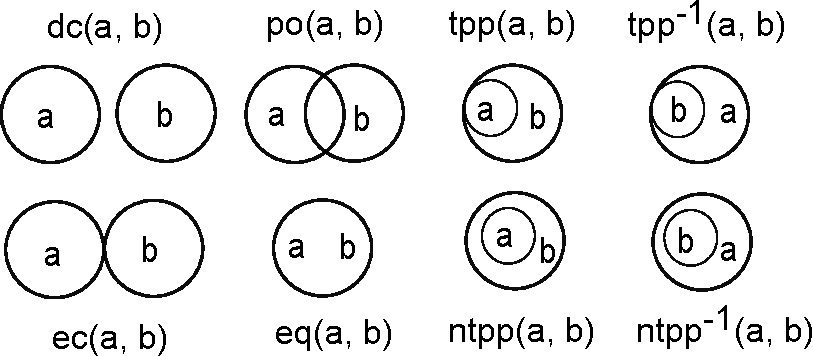
\includegraphics[width=43mm]{rcc8-primitives}}
 \hspace{7 mm}
 \subfloat[SCC]{\label{SCC-calc}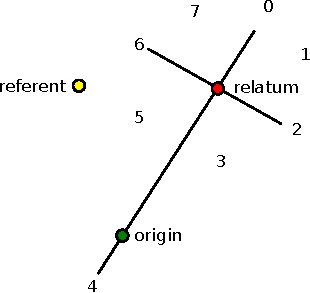
\includegraphics[width=34mm]{scc}}
  \hspace{7 mm}
 \subfloat[OPRA$_{2}$]{\label{OPRA-calc}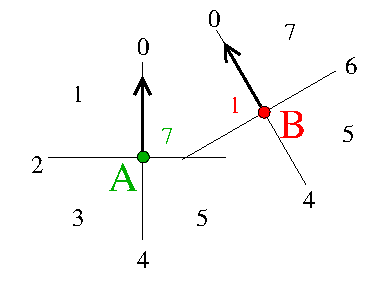
\includegraphics[width=43mm]{OPRA2_Example}}
 \caption{Qualitative Spatial Calculi}
\label{Qualitative Spatial Calculi}
\end{figure}

RCC defines eight topological relationships over regions: disconnected, partial overlap, externally connected, equals, non-tangential proper part, inverse non-tangential proper part, tangential proper part, and inverse tangential proper part. Refer to figure \ref{RCC-calc} for an illustration of these relationships. Axiomatic rules of jointly exhaustive, mutually disjoint and pairwise disjoint (JEPD) enforce the spatial uniques of each relationship \cite{Randell92aspatial}. For example, two regions can \emph{not} be partially overlapping and disconnected at the same point in time. Additionally, composition tables define the set of realizable spatial configurations for a collection of regions. For example, if region \emph{A} is inside region \emph{B} and region \emph{B} is inside region \emph{C}, then region \emph{A} must also be in region \emph{C}.

Orientational relationships can be broken down into intrinsic and extrinsic spatial relationships. Extrinsic relationships are defined by  an external reference point. This type of orientational relationship is characterized in the SCC, in which an external reference point is used to relate two objects together. Figure \ref{SCC-calc} illustrates the SCC partitioning of space for three points, \emph{A}, \emph{B}, and \emph{C}. In this example, \emph{C} is related to \emph{A} through \emph{B}, and has an SCC 2 relationship. 

Intrinsic relationships are defined by an internal perspective. This type of relationship is characterized in OPRA, in which the relationship of an external object is defined by the internal direction of the observing object. Figure \ref{OPRA-calc} shows the relationship between two points, \emph{A} and \emph{B}. In this example point \emph{B} has an OPRA$_{2}$ relationship with \emph{A} of \emph{7} and point \emph{A} has an OPRA$_{2}$ relationship with \emph{B} of \emph{1}. 

As with RCC, axiomatic rules of JEPD and composition tables enforce spatial properties of uniqueness and composition for these two orientational calculi.

\section{Constraint Logic Programming}
Constraint Logic Programming (CLP) combines logic programing with constraint solving \cite{GavanelliCLP} \cite{WallaceCLP} \cite{Jaffar:1987:CLP}. Logic programming is based on a declarative semantic in which programs are defined in terms of \emph{what} should be computed instead of \emph{how} it should be computed (i.e. procedural style). In this regard, a logic programing language relies on built-in search and unification algorithms to solve logic based formula. At its essence, logic programming can be viewed as a basic form of constraint solving \cite{GavanelliCLP}. 

Prolog is one of the most well known and used logic programming languages. It is based on predicate logic, unification, logic conjunction, and depth-first search \cite{Sterling:1986}. From a constraint perspective, Prolog solves constraints over the set of uninterpreted structures, i.e. Prolog's unification algorithm works entirely on a syntactic level. What this means is that Prolog does not internally 
represent data beyond its syntax and can only unify terms based on this. Take for example the arithmetic expression 5 + 1 = 6, where in Prolog this expression will fail because equality is true only on the syntactical level, i.e. 5 + 1 = 5 + 1.  

Constraint solving techniques can help logic programming by increasing the expressiveness of the language beyond the syntactic. In general, constraint solving is based on constraints, which are simply restrictions over the values a set of variables can bind to. For specific constraint solvers, the variables and the constraints over the variables are based on a specific domain, such as arithmetic expressions, boolean logic, etc., which encode the semantics and unification algorithms for solving the logical formula directly in a logic based language. In the example above, a constraint solver for arithmetic expression would be able to resolve the expression 5 + 1 = 6 as true because it knows directly about the semantics of addition and equality. 

Building new constraint solvers is laborious because it typically requires hard-wiring the constraint solver into the complier or interpreter \cite{GavanelliCLP}. The use of Constraint Handling Rules (CHR) can help this process by providing a high level programming framework designed for the implementation and integrate constraint solvers into logic based languages. The aim is to ease the process of building constraint solvers in terms of defining a new domain of constraints and integrating these constraints into a logic programming framework \cite{CHR} \cite{Fruhwirth94}. CHR works by using logic based rules that rewrite constraints via simplification and propagation rules and constraints are solved by continually rewriting constraints until they are in a solvable form. Because these rules are based on logic themselves it integrates seamlessly into other logic based frameworks. 


%To solve this task it is unnecessary to have knowledge about the precise spatial characteristics of the room -- such as the size, shape, and weight of objects, metric measurements such as distance, etc. -- because the solution does not require an absolute location of the chair. Rather, a qualitative description of the room in terms of the orientational relationships between objects and the observer (\emph{left-of, righ-of, behind}) within the room should suffice. A specific qualitative description for this problem could be, the chair is \emph{left-of} the doorway and \emph{behind} the desk. This problem was solved from a qualitative spatial perspective by abstracting away the insignificant details and focusing on the aspects of space that are necessary for the problem domain. 

%As with any abstracting mechanism, QSR deals with high level abstractions by hiding away unnecessary details while preserving important domain specific aspects

%The advantages to QSR include reducing the search space of the spatial environment, using a higher level of abstraction that is closer to the conceptual representation of space that humans use...


\chapter{Related Works} \label{relatedwork}
This Chapter presents the related work for this thesis. There is a large body of research on tools for conceptual design assistance. The related works that will be discussed in this Chapter have been narrowed to tools that provide assistance to a designer and use spatial reasoning as the basis of its design analysis.


\section{Intelligent Critic System}
The intelligent computer-aided architectural design system (ICAAD) \cite{IntelligentCritic} is a tool that evaluates architectural floor plans based on government regulations and interior design guidelines. The research here focuses on the spatial representation model for architectural designs in the context of checking for requirements. In this respect, ICAAD represents designs in an object oriented hierarchical model, which is grounded to architectural containment relationships, i.e., windows are contained by rooms, rooms are contained by apartments, and apartments are contained by buildings. Various architectural entities, such as rooms, windows and furniture are all represented individually as ICAAD objects in the hierarchical structure. Each ICAAD object is responsible for storing spatial data about the entity, including dimension, shape, and direction. Spatial relationships between entities, such as proximity and visibility, are extracted from the spatial data and are represented as a network, which connects entities together based on their spatial relationships. 

ICAAD uses Prolog's inference engine to match design rules (i.e., government regulations and interior deigns guidelines) against the ICAAD representation model. Violations are detected when a spatial relationship between entities are matched to a design requirement rule in Prolog.


\section{The Architect's Collaborator}
The Architect's Collaborator (TAC) \cite{KoileTAC} is a design support system that evaluates designs based on architectural qualities and provides recommendations to the designer with respect to these qualities. Within TAC, architectural qualities refer to experiential aspects of a design such as \emph{openness} and \emph{privacy}. The main contribution of TAC is that it evaluates designs based on architectural qualities and provides recommendations for improving the design.

For example, a designer might use TAC to evaluate a kitchen based on it being \emph{visibly open}. TAC evaluates this quality (visibly open) based on a pre-defined spatial characteristic of the design, in this case, the percentage of this room (kitchen) that is visible from an adjacent room. A room is considered by TAC to be visibly open if the result of the calculation is above a certain threshold. If it is below the threshold, TAC will provide recommendations to the designer to help increase the visual openness of the kitchen. 

The main drawback to TAC is its use of `black box' spatial reasoning. From the example above, TAC directly maps the architectural quality of visual openness to a specific low level geometric characteristic of the design. This type of spatial reasoning if very specific to the definition of the problem, therefore making it difficult to expand upon. 


\section{ICADS}
The Intelligent Computer-Aided Design System (ICADS) \cite{ICADS} is a collaborative design support tool that assists a designer by providing functional based analysis of a design. The tool provides analysis to a designer based on several different aspects, such as lighting, noise insulation, climate control, energy conservation, space layout, and construction costs. The focus of this research is on developing a series of knowledge based software agents that collaborate within ICADS to make recommendations to the user. 

\section{SEED}
The Software Environment for Supporting the Early Phases in Building Design (SEED) \cite{SEEDS} project is a framework that supports an architect during the entire architectural design process. Specific to the work done in this thesis, the SEED project introduced the idea of using constraints to represent design knowledge in order to automatically generate floor layouts. 

Within the SEED project, design knowledge is partitioned into two categories: design units and functional units. Design units represent the spatial and physical elements of a building. Functional units represent design requirements that constrain design units based on spatial attributes such as shape, size and placement, and non-spatial attributes such as material make-up. 

Given a design, the SEED project automatically generate possible floor plans that adhere to all of the design requirements, given a set of design and functional units. The main contribution of this work is that the system utilizes the constraint solving abilities in a CLP framework to autonomously find design layouts that meet the design's requirement specifications.


\section{Interior Design Configuration for a Virtual \newline Environment}
Calderon \emph{et. al} \cite{Calderon06} proposed a system that automatically configures an indoor virtual environment, with respect to the placement interior design elements, by specifying the design problem in terms of spatial constraints. The system works by solving constraint satisfaction problems as specified over the space of the virtual environment.

The spatial constraint problems are defined as follows: Given a space for the virtual environment represented as a discrete Cartesian grid, a set of interior design objects (desks, chairs, lamps, etc.), and a set of spatial constraints over the design objects (e.g., a desk should be at least four meters from a power outlet), the system searches for viable locations for each object within the virtual environment such that all of the spatial constraints are satisfied. 

The contribution of this work lies in the use of spatial constraints for reasoning about virtual environment design. However, the work here is preliminary and has several shortcomings. To begin with, the virtual environment used in this system is limited to a rectangular grid represented by discrete Cartesian coordinates. This means all spatial reasoning is over the discrete finite integer domain. Additionally, the expressiveness of the spatial constraints is limited. For example, topological relationships are defined over rectangles and points with respect to the point being inside or outside the rectangle. No consideration is made for orientation, or objects with richer geometries than points and rectangles.

\section{Others}
The following research presents other related work that is similar to the work in this thesis, but differ from the primary works discussed above because they are less established work.

Bhatt \emph{et. al} proposed a system in \cite{BhattDH09} that validates a designer's conceptual requirements against an architectural design in the context of Smart Homes. This research introduced the idea of modeling the artefactual space of the design's structural elements and uses topological reasoning to detect design inconsistencies per a set of design requirements.

Key proposed a descriptor language \cite{Key} that defines architectural qualities from a computational perspective. The work here is quite similar to the work in this thesis with regards to the approach that architectural qualities emerge from spatial configurations of design entities and that these qualities can be spatially characterized. The language defines architectural descriptors for concepts such as enclosure, continuity, and spaciousness and does so by interpreting the descriptor in terms of spatial properties. However, the approach here lacks the integration of a qualitative intermediate layer between the high level concepts and low level geometries and instead uses a more direct approach to geometric and spatial reasoning.

Borrmann introduced the idea of including predefined spatial constraints directly into a standard building production model, the Industry Foundation Classes (IFC) \cite{IFC}, to detect constraint violations \cite{Borrmann}. This proposal focuses primarily on the definition and integration of spatial constraints into the IFC data model and also provides some discussion on how these spatial constraints might be checked in such an environment. While similar to CRR, this proposal's approach is focused on the integration of spatial constraints into a specific building model (IFC) and does not go into the process of generating the spatial constraints from the spatial configurations of a design. 


\section{Discussion}
Table \ref{related works table} shows the high level objectives of each tool discussed in this section. This Table includes requirements checking, design evaluation, and automatic floor plan configuration. Despite the differences, each system provides design assistance at a conceptual level.

\begin{table}[H]
  \begin{center}
   \scalebox{0.87}{
  \begin{tabular}{ | r | c | c | c | c | c | c | c |}
    \hline
    & CRR & ICAAD & TAC & Bhatt & ICAD & SEED & CLP \\ \hline
    requirement checking & X & X &  & X &  &  & \\ \hline
    design evaluation &  &  & X &  & X &  & \\ \hline
    automatic floor plan configuration &  &  &  &  &  & X & X \\ \hline
   \end{tabular}
   }
  \end{center}
\caption{Related Work System Objectives}
\label{related works table}
\end{table}   

Out of this group the ICAAD tool has the most in common with the CRR. Both systems provide a framework for checking design requirements using qualitative spatial relationships. Despite these similarities, there are many differences. ICAAD focuses on the spatial representation model for designs in the context of requirement reasoning and gives little attention to or discussion of the underlying techniques for spatial reasoning and spatial abstraction, as is the focus in the CRR. While the ICAAD approach allows the system to reason automatically over the entire design, it does so by relying on the underlying 'black box' spatial reasoning. Extending 'black box' reasoning can be difficult because spatial functions are built only to solve a specific problem. On the other hand, the CRR uses general qualitative spatial reasoning and formal spatial calculi to reason over architectural designs. The advantages to this approach is that the reasoner is extensible, i.e., it is easy to build new design requirements by using the existing services of the spatial reasoners.  

Table \ref{functionality table} shows various features provided by the related works. This includes whether the tool supports reasoning about experiential qualities (openness, privacy), and artefactual extension (operational / functional space), if the tool incorporates spatial representation and reasoning techniques and formal qualitative spatial calculi, if the system provides the user with feedback or recommendations based on design analysis, and if the system uses constraint based reasoning.

\begin{table}[t]
  \begin{center}
  \scalebox{0.87}{
  \begin{tabular}{ | r | c | c | c | c | c | c | c |}  
      \hline
      & CRR & ICAAD & TAC & Bhatt & ICAD & SEED & CLP \\ \hline
    experiential qualities & X & X & X &  &  &  & \\ \hline
    artifactual extension & X &  &  & X &  &  &  \\ \hline
    spatial representation and reasoning & X & X & X & X & X & X & X \\ \hline
    formal qualitative spatial calculi & X &  &  & X &  &  & \\ \hline    
    feedback / recommendation &  &  & X &  & X &  &  \\ \hline
    design evaluation &  &  & X &  & X &  &  \\ \hline
    constraint based reasoning & X &  &  &  &  & X & X \\ \hline
  \end{tabular}
  }
  \end{center}
\caption{Related Work Features}
\label{functionality table}
\end{table} 

The CRR provides provides five of the seven features. It does not provide feedback to the user and it does not evaluate a design based on metrics. The intention for this version of CRR is to provide a solid framework for spatial reasoning over architectural designs and requirement reasoning. Future versions of the tool might incorporate these aspects. 

Table \ref{spatial table} shows the spatial reasoning capabilities for each system. It includes spatial reasoning for topological relationships, orientation (intrinsic and extrinsic), distance, and metric. Metric relationships refer to quantitative geometric functions such as the calculation of length or area.  

\begin{table}[H]
  \begin{center}
  \scalebox{0.9}{
    \begin{tabular}{ | r | c | c | c | c | c | c | c |}
     \hline
     & CRR & ICAAD & TAC & Bhatt & ICAD & SEED & CLP \\ \hline
     topology & X &  & X & X & & X & X  \\ \hline
     intrinsic orientation  & X & X &  &  &  &  &  \\ \hline
     extrinsic orientation & X &  &  &  &  &  &   \\ \hline
     distance  & X & X & X &  &  & X & X  \\ \hline
     metric & X & X & X &  & X & X & X  \\ \hline
   \end{tabular}
  }
  \end{center}
\caption{Related Work Spatial Reasoning}
\label{spatial table}
\end{table}

The CRR is the only tool in the group which provides support for every type of spatial reasoning. Additionally, it is the only system that does so using formal qualitative spatial reasoning and representation techniques. This is one of the main advantages of the CRR. Using a broad variety of of spatial relationships (topological, orientational, distance, metric) the CRR provides flexibility and a rich set of spatial relationships to build design requirements. This is important because the spatial configurations that make up a building are complex and need flexibility in terms of the way they are characterized and reasoned over. 

%the systems are all bound by a higher objective to provide computational assistance to an architect during the design process and specifically, in the context of conceptual design formalization and reasoning.

%s based on formal qualitative spatial calculi (\cite{scc} \cite{opra} \cite{topolog}), formalization and spatial interpretation of architectural concepts (i.e. experiential and spatial qualities found in architecture), and the abstraction of CAAD based geometric representations into the qualitative spatial domain.



\chapter{The Conceptual Requirements Reasoner} \label{ccr}
This Chapter is an introduction to the Conceptual Requirements Reasoner (CRR), a framework for validating conceptual design requirements against CAAD-based design plans. The Chapter begins by presenting the problem statement that is addressed in this thesis. The next section presents the scope and contribution of the thesis. The final section introduces the high level design and implementation of the CRR in the context of the problem statement.
 

\section{Design Problem}
The field of Spatial Computing for Architectural Design \cite{bhatt-spatial-computing} investigates the computation apparatus that is necessary to represent and reason about architectural form and function from multiple levels of abstraction: \emph{conceptual}, \emph{qualitative}, and \emph{quantitative}. At the conceptual level the architect perceives the design at a high level of abstraction. For example, at this level the architect would think in terms like spaciousness, privacy and continuity. At the quantitative level the architect engages the design at a low level of abstraction. Now the architect considers concrete, physical aspects of the design. These include the geometric shape and spatial location of the design's structural form. These levels of abstraction are referred to in this thesis as the architectural design hierarchy, where the top of the hierarchy corresponds to the conceptual (design), the middle corresponds to the qualitative, and the bottom corresponds to the quantitative. 

Applying the architectural concept of spaciousness to the architectural design hierarchy will show how high level concepts are connected to low level spatial quantities. In this example, the concept of spaciousness conveys an experiential quality of the design such as the feeling of openness. Such an experiential quality emerges from of the spatial design patterns of the building's physical form. In other words, the location and placement of architectural entities such as walls, ceilings, windows, and doors, and their spatial relationships as they define the size and shape of rooms and spaces, directly affect the experiential quality of openness. In general, changes in the spatial patterns at the quantitative level affect the experiential qualities of the design at the conceptual level. Figure \ref{multi-perspective-reps} illustrates this concept in which the features of the design at the conceptual level emerge from its spatial environment at the quantitative level via spatial patterns on the qualitative level. 

\begin{figure}[t]
\centering
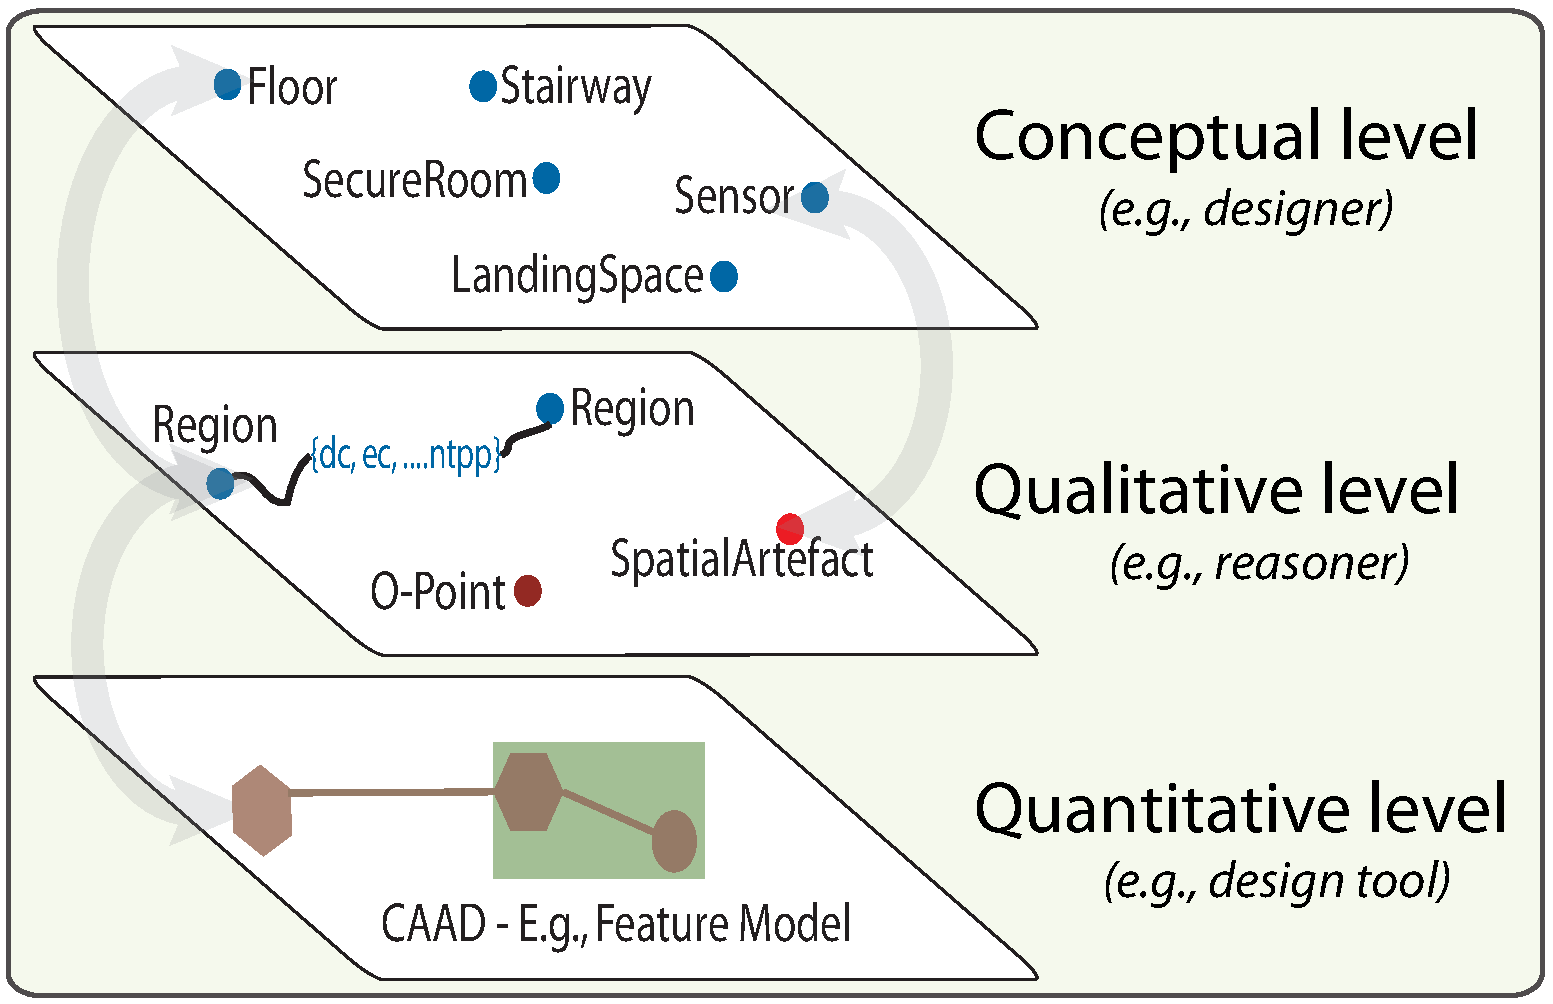
\includegraphics[width=95mm]{multi-perspective-reps}
\caption{Architectural Levels of Abstraction - Source \cite{bhatt-spatial-computing}}
\label{multi-perspective-reps}
\end{figure}

Unfortunately, state-of-the-art CAAD programs \cite{ArchiCAD} do not support the representation of and reasoning about architectural design at a conceptual level. This happens because the CAAD-based spatial representation model is encapsulated at the quantitative level of the architectural design hierarchy, which lacks the semantics necessary for representation and reasoning at higher levels of abstraction. While this model is well suited for certain design tasks, such as the building of an accurate blueprint of the design, it does not support other architectural design processes that require reasoning at a higher level of abstraction. These include design conceptualization, requirements reasoning and functional specification, to name a few \cite{bhatt-spatial-computing}. 

Take for example the tasks an architect might face during the design conceptualization phase of a museum, including, among other things, defining high level functional and aesthetic requirements of the museum's design. The following descriptions of the \emph{Museu Calouste Gulbenkian} in Lisbon, Portugal exemplifies this phase \cite{Tostoes}:
\begin{quote}
\emph{The current topographic conditions of the site, where the larger trees are located in an area that is more elevated than the whole northern rim of the plot, made it possible to install a huge underground floor in the already existing depression, whose covering creates a gentle artificial elevation that perspectively accentuates and enhances the whole architectural composition. The distribution of the construction volumes fundamentally followed a desire for horizontality, allowing one to read the continuity of the green space beyond the construction and in all directions.}
\end{quote}
\begin{quote}
\emph{This sober, rational and markedly horizontal structure is distinctive for its laminar exterior, its modular repetition, austere design and the hard quality of the materials which shape it, concrete and glass.}
\end{quote}
Environmental aspects of the museum's design, such as these expressed in the above descriptions, encompass high level spatial design patterns that are identified at the design conceptualization phase. Because CAAD-based programs do not represent the design at a level of abstraction that is required to express these conceptualization, it is therefore incapable of providing the designer with assistance during this phase of the design process.

Design reasoning at a conceptual level, such as the example above, requires the underlying model representation semantics at the same level of abstraction. In this regard, the design semantics at the conceptual level involve abstractions over architectural entities such as rooms, floors, buildings, doors, and walls, along with the relationships they share between each other, both spatially (facing, near-to, across-from, connected-to) and non-spatially (material composition, lighting attributes, and load bearing qualities). Conversely, the underlying model representation semantics of CAAD-based program are based on spatially general and low level geometric primitives of points, lines, and polygons that lack the notions at the higher levels of the architectural design hierarchy. Whereas an architect might conceptualize the design of a museum in terms such as galleries and the relative placement of objects within each gallery, e.g., ``the statue is on the \emph{left-hand-side} of the gallery as one enters from the main doors,'' the process of building the museum in a CAAD-based program restricts the architect to using points, lines and polygons. 

The \emph{semantic gap} exemplified between the conceptual and quantitative levels of the architectural design hierarchy is the crux of the problem being addressed in this thesis. The following section introduces the scope of this thesis by narrowing the focus of the thesis to conceptual requirements reasoning, outlines the approaches taken towards this goal, and presents the thesis's main contributions. 

%The design semantics at the quantitative level do not represent the design at a level of abstraction that is need to reason at a conceptual level.

%For example, it is possible to reason about the geometric properties of a design in terms of the size, shape, and location of architectural entities given the CAAD-based representation semantics of space. At this level of reasoning, the reasoner and the underlying representational model are both ground to the same level of abstraction, namely the quantitative semantics of polygon, lines and points. 

%Unfortunately, reasoning at more abstract levels, involving conceptual design semantics such as visibility, continuity, and enclosure, or spatial qualities such as facing, across-from, and near-to, breaks down because there is a \emph{semantic gap} between the levels of abstraction of the reasoning queries with the underlying representation.



\section{Scope and Contributions}
The objective of this thesis is an initial step towards building a framework that bridges the gap between a design's conceptual features to its real world quantitative representation (i.e., how it is represented in a CAAD-based program). Specifically, the framework, referred to as the Conceptual Requirements Reasoner or CRR, does this in the context of conceptual requirements validation. Conceptual requirements validation involves checking that the underlying spatial structures of a design, in the quantitative representation, are consistent with its conceptual features as they are specified by an architect. Towards this goal the following objectives have been identified as crucial:
\begin{itemize}
\item the identification, formal modeling, and spatial interpretation of architectural concepts
\item the qualification of CAAD-based spatial models, and
\item the use of qualitative spatial representation and reasoning techniques to link high level concepts to low level spatial quantities  
\end{itemize}

To address these objectives, this thesis follows the approach introduced by Bhatt and Freksa \cite{bhatt-spatial-computing}, with regards to Spatial Computing for Architectural Design. This thesis does so by following the design space hierarchy as illustrated in Figure \ref{multi-perspective-reps}, in implementing the CRR. The main contributions in this respect are identified here:
\begin{itemize}
\item the implementation of a framework that validates conceptual design requirements against a CAAD-based spatial representation
\item the identification of a set of QSA and architectural concepts
\item the development of a multi-hierarchy that maps QSA and architectural concepts to spatial patterns in the qualitative level
\item the implementation of spatial constraint solvers that qualify CAAD-based spatial models
\item the development of a real world museum case study that demonstrates the applicability and effectiveness of the CRR in validating museum design requirements
\end{itemize}


The following section introduces the high level design and implementation of the CRR with regards to the scope and contributions identified in this section. 

%  - main problem: how to go from high level conceptualization of a design to low level quantitative level
%  - solution: use intermediate spatial level: i.e. qualitative space
%  	  - Break down design / architectural domain into spatial / design hierarchy
%         - design space
%         - quality space
%         - quantity space
%         + each level of hierarchy is responsible for a level of abstraction
%         + mapping between each level bridges gap between concept and quantity
%         	- design to quality downward connected via spatial definition (interpretation) of design concept into qualitative spatial relationships
%         	- quality to quantity upward connection via qualification
%         + complexity of spatial reasoning / representation of design is hidden from architect

%The main problem being addressed in this thesis is how to validate conceptual design requirements in a practical design workflow involving a CAAD based design representation. As discussed in the previous section, designs are represented quantitatively in CAAD based systems using spatial primitives of point, lines, and polygons that do not incorporate the semantics needed for reasoning at higher levels of abstraction, such as conceptual requirements validation. 

%Given the need to bridge the gap between the conceptual and the quantitative levels of the design hierarchy in this context the following issues have been identified as crucial:

%focuses on supporting a designer by validating conceptual requirements against a work-in-progress design from a CAAD-based system. The framework built for this thesis is referred to as the Conceptual Requirements Reasoner or CRR.
     
      
%This representation allows an architect to validate a work-in-progress design from a conceptual and qualitative perspective against the physical and precise real world geometrical representation of the design \cite{Bhatt}.

%The crux of this is that it bridges the gap between the quantified geometries and the functional / qualitative requirements of the design, thus allowing the reasoner to validate a high level requirement against its precise geometric representation. 


\section{Design and Approach}
The design and implementation of the CRR is based on the design hierarchy as illustrated in Figure \ref{hierarchy no-links}. Following this structure, the CRR breaks down the problem into a design space module, quality space module, and quantitative space module. At the top level, the design space model is responsible for the representation of and reasoning about architectural concepts and QSA. This module will be used as the basis for building conceptual requirements. The middle level of the hierarchy, the quality space module, represents the design based on qualitative spatial relationships of orientation, topology and distance. Within the CRR, qualitative spatial relationships are defined using formal qualitative spatial calculi such as the Region Connection Calculus for topological relationships, the Single Cross Calculus for extrinsic orientational relationships and the Oriented Point Relational Algebra for intrinsic orientational relationships. The lowest level of the hierarchy, the quantity space module, is responsible for representing the design in terms of its physical and artefactual form.

\begin{figure}[t]
\centering
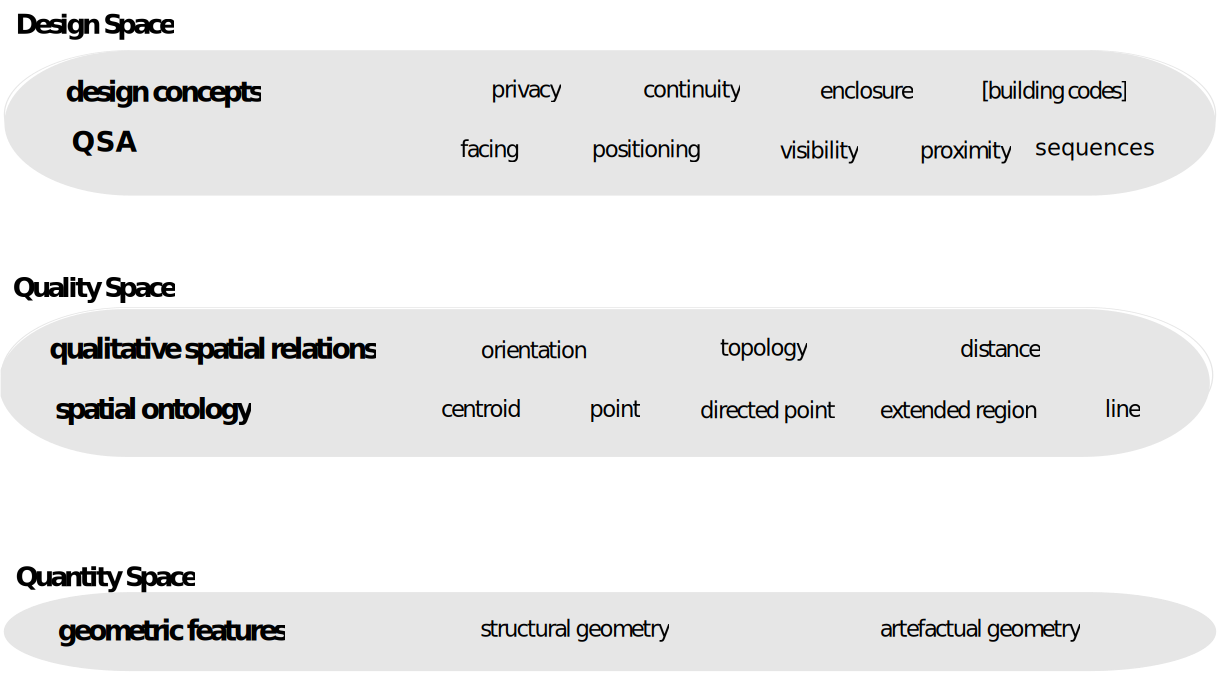
\includegraphics[width=140mm]{spatial-qualities-hierarchy-nolinks}
\caption{Design Space Multi-Hierarchy}
\label{hierarchy no-links}
\end{figure}

Given these three modules, the main issue now becomes how each level interfaces with the others. In other words, how do concepts in the design space relate to qualitative spatial relationships in the quality space, and similarly, how do qualitative spatial relationships in the quality space relate to geometric objects in the quantity space? At the core of this is the qualitative module, an intermediary layer that interfaces between the design and quantitative modules. 

Architectural concepts and QSA are linked to qualitative spatial relationships of orientation, topology and distance by explicit characterization. In other words, concepts in the design space are explicitly defined by qualitative spatial relationships. For example, the architectural spatial quality of positioning, where objects can be spatially situated at the same or opposing sides of a room, is defined by extrinsic orientational spatial patterns using the OPRA calculus. Chapter \ref{design space} will go into further detail regarding the specific spatial interpretation and characterization of each concept and QSA as identified in the thesis.

\begin{figure}[t]
\centering
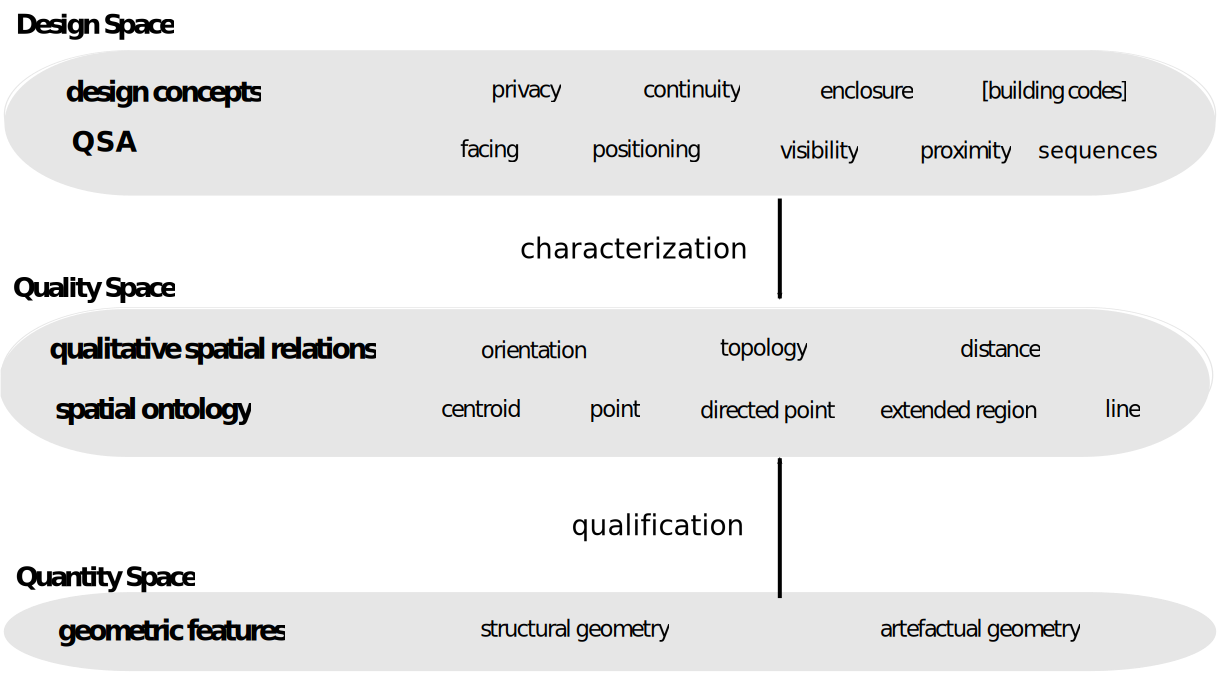
\includegraphics[width=140mm]{spatial-qualities-hierarchy}
\caption{Design Space Multi-Hierarchy}
\label{hierarchy}
\end{figure}

The geometric quantities in the quantitative level are connected to the qualitative spatial relationships in the qualitative level through spatial abstraction and qualification. Through this process the spatial quantities of the design are connected to qualitative spatial relationships. Chapter \ref{representation and reasoning}  will go into the details regarding the CRR's underlying spatial representation structure at the quantitative level and the spatial reasoning necessary to spatially abstract and qualify the quantitative representation.  

\begin{figure}[t]
\centering

\includegraphics[width=100mm]{design}
\caption{CRR Implementation Design}
\label{crr design implementation}
\end{figure}

The implementation of the CRR is broken down into three modules as identified in the design hierarchy, and is illustrated in Figure \ref{crr design implementation}. The top level module is where architectural concepts and QSA are defined in terms of qualitative spatial patterns and is the interface through which  users will query the CRR. The quantitative space module models the design's physical form and artefactual extension. The data at this level is imported from a multi-modal access framework \cite{carl} based on the IFC standard for CAAD-based systems. The qualitative space module is responsible for the spatial abstraction and qualification of the quantitative model and is implemented as a series of spatial constraint solvers for topological, orientational, and distance reasoning. 

From a user perspective, the CRR provides the user with design assistance in validating requirements for a work-in-progress design. The CRR does this this by providing a query engine that allows a designer to validate conceptual requirements. For example, a designer is provided with a set of architectural concepts and QSA, which the designer uses to construct queries to the CRR. So if a designer wants to check if a door and window are facing each other (as might be a requirement for air circulation purposes) the designer can make the following query to the CRR:
\begin{verbatim}
    ?- facing(door, window).
\end{verbatim} The CRR will respond \emph{true} to the query if the door and window are facing each other and respond \emph{fail} if they are not.

%The conceptual and qualitative levels of the design hierarchy are connected through an individual mapping of each concept and spatial quality to qualitative spatial design patterns.

%One interpretation of this quality is based on extrinsic orientational spatial patterns that are based on qualitative spatial relationships. In this case, the orientational relationships of the structural form define the design's positioning qualities. 

%The concepts and spatial qualities in the design space are connected to qualitative spatial relationships in the qualitative space through a process of spatially interpreting and characterizing design concepts and spatial qualities individually.

%  - Design
%      - based on multi-hierarchy
%      - design space
%      		- concepts / qualities explicit characterization
%      		- downward connection via spatial interpretation 
%      - quality space: 
%       		- qualitative spatial constraint solvers
% 				- orientation, topology, distance
% 			- upward connection via spatial abstraction 
%      - quantity space
%      		- physical, artefactual     
%  - introduction to implementation
%      - declarative framework / clp
%      - details will be discussed in subsequent chapters

%The design multi-hierarchy developed in this section is built on the mapping of the design problem into a design space, a quality space, and a quantity space. At the highest level, the design space involves the architectural design semantics (architectural concepts) and qualities (qualitative spatial attributes found in architecture) that emerge in architecture. At the lowest level, the quantitative space involves the precise geometries of the architectural structures found in the design. The qualitative space mediates between the abstractions of the design layer and the concreteness of the quantitative later using qualitative spatial representation and reasoning.

%Figure \ref{hierarchy} shows the design multi-hierarchy used in the DSpace reasoner. Conceptual design requirements are built from the architectural concepts and qualitative spatial attributes found in architecture (QSA) of the highest level of the multi-hierarchy. Within the multi-hierarchy, architectural concepts are built using QSA, but are not limited to only these, spatial relationships of orientation, topology, and distance can be used, as well as other geometric primitives such as area, angle, and length measurements. QSA are defined by the qualitative spatial relationships of orientation, topology, and distance. These qualitative spatial relationships emerge from the quantitative, physical, and artefactual geometries of the the design. TBD: physical structures define the way the architecture is experiences and influences the functional / performance of the design from a conceptual design perspective. 

%Prolog facts make up a factbase that stores a table of architectural entities with their architectural types (e.g., wall, door, window, desk, etc.). Each architectural entity in the design has a single entry in the factbase. The factbase is instantiated automatically during the import process from a CAAD based representation. This factbase will be used throughout the DSpace reasoner to  verify an entity exists in the design and links it to its architectural type. The following Prolog code shows two instantiated facts (predicates) for a doorway, and a window. 


\chapter{Design Representation and Spatial Reasoning} \label{representation and reasoning}
This Chapter presents the quantity and quality modules of the CRR. For the quantity module, this Chapter present the internal architectural design representation model. For the quality module, this Chapter presents spatial constraint solvers that are used by the CRR to qualify spatial relationships. Additionally, this chapter presents each module in the context of the declarative programming paradigm used for the implementation of the CRR, namely Prolog and Constraint Logic Programming (CLP). 

This chapter has two sections. The first section presents the internal architectural design representation structure and shows how it is implemented in Prolog. The second section looks at the spatial constraint solvers and shows how each is implemented in CLP.

\section{Design Representation}
The CRR represents two distinct aspects of a design. It represents the design's physical form and non-physical artefactual extensions. The physical form pertains to the precise geometric data that defines the design's architectural entities with regard to layout, location and shape. In this thesis architectural entities refer to the structural elements of walls, doors, windows, slabs, stairs, and columns. Artefactual extension pertains to the non-physical but geometric data that defines the functional characteristics of architectural entities, such as the space used by a person to operate a doorway.

The physical representation of the design is automatically imported into the CRR from a multi-modal spatial data access framework \cite{carl} built by the DesignSpace project \cite{DesignSpace}. For each architectural entity, the CRR imports the structural geometric coordinate data, as it is represented in a CAAD-based program, and a unique identifier referred to in the CRR as the \emph{crr\_id}. Currently, artefactual extensions are manually imported, but the intent for future versions is to automate this directly from the multi-modal spatial data access framework.  

The remainder of this section is broken up into three subsections. The first subsection looks at the physical representation structure. The second subsection looks at the artefactual representation structure. The third subsection looks at how both are implemented in the CRR.

\subsection{Physical Design Representation}
The CRR represents a design's physical form in terms of geometric features of layout, shape, and location. Each architectural entity is represented in the CRR as a polygon made up of Cartesian points that correspond to the physical dimensions (length, width, shape) of the entity as is occurs in the real world. The physical representation of the design is analogous to the design perspective that is represented by CAAD programs. 


\subsection{Artefactual Design Representation}
An artefactual extension is a non-physical, spatial extension of an architectural entity that pertains to a specific functional quality. While an artefactual extension does not have a physical manifestation, it is none the less an important aspect of the design representation model because it affects the functionality and performance of a design from an experiential perspective. 

There are three types of spatial artefacts identified by Bhatt\cite{BhattDH09} that are represented in the CRR: \emph{operational space}, \emph{functional space}, and \emph{range space}.


\begin{figure}[H]
 \centering
 \subfloat[Artefactual Extensions]{\label{Artefactual Extensions}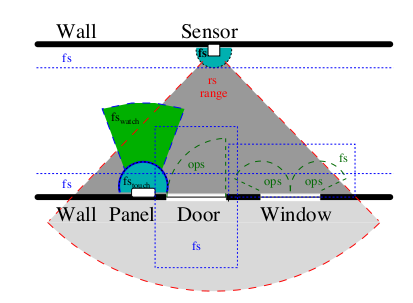
\includegraphics[width=60mm]{artefacts2}}
 \hspace{7 mm}
 \subfloat[Functional Space (FS), Operational Space (OS), Range Space (RS)]{\label{artefactual-extensions2}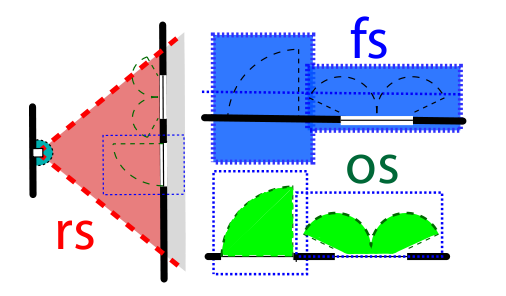
\includegraphics[width=70mm]{artefacts}}
 \caption{Artefactual Extension, Source \cite{bhatt-spatial-computing}}
\label{artefactual-extensions}
\end{figure}

The operational space encompasses the region of space required by an object to preform its function. For example, the operational space of a door is the area in which a door can occupy during its operation, opening and closing (see figure \ref{artefactual-extensions2}). This space is dynamic in the sense that it represents the configurable space of the physical doorway. 

The functional space encompasses the region of space that is required for an object to function itself or the space for a person to operate an object. For example, the functional space of a doorway is the total area needed for a person to operate, open and close, as well as any additional space need to navigate entirely through the doorway (see figure \ref{artefactual-extensions2}).

The range space pertains to a region of space that encompass the range of a sensor (i.e., camera, motion sensor). For example, the range space of a camera is defined by its depth of field and angle of view. It represents the total space that is under surveillance of the camera (see figure \ref{artefactual-extensions2}).

\begin{figure}[H]
\centering
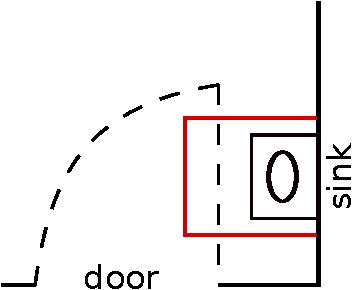
\includegraphics[width=50mm]{door-sink}
\caption{Operational Space Interference}
\label{door-sink}
\end{figure}

Each artefactual extension is represented in the CRR as a polygon that corresponds to its spatial dimensions.

Artefactual extensions directly affect the experiential quality of a design. For example, a sink in a bathroom has a functional space, the space a person occupies while washing his/her hands at the sink. If this space interferes with (i.e., topologically overlapping) the functional and/or physical space of a doorway, this will cause a circulation problem when both the doorway and sink are simultaneously being operated, because it will cause a collision between the person washing his/her hands and the doorway. In this example, the functional aspects of the bathrooms design with regard to the mitigation of circulation problems is directly influenced by the spatial configuration of the non-physical artefactual extensions of the design. It should be noted that this type of occurrence can not be modeled in current CAAD-based program because they do not represent artefactual extension.


\subsection{Implementation}
Within the CLP framework of the CRR, the physical and artefactual representations are implemented as factbases and rulebases. There are two factbases that are in memory database-like structures. One of these factbases is used as a catalog, which relates each architectural entity to its architectural type (wall, window, door, room, interior design object, etc.) via its \emph{crr\_id}. Each entry in this factbase is a Prolog predicate of the form $architectural \mathunderscore type(crr \mathunderscore id, type)$.
\begin{verbatim}
   architectural_type(door42, door).
   architectural_type(wall49, wall).
\end{verbatim} The other factbase is used as a linking table to relate architectural entities together based on containment relationships. The CRR represents two types of containment relationships. The first is the containment relationship between rooms and architectural entities and interior design elements. This containment relationship defines which architecural entities and interior design elements are contained in which rooms. In a specific design, desk2 is contained in room6, and wall5 in contained by room6. Each containment relationship is implemented as a Prolog predicate of the form $contained\_room(contained \mathunderscore crr \mathunderscore id, containing \mathunderscore crr \mathunderscore id)$.
\begin{verbatim}
   contained_room(desk2, room6).
   contained_room(wall5, room6).
\end{verbatim} The second containment relationship is between doors / windows and walls. This containment relationship defined which doors / windows are contained by which walls. For example, door42 is contained in wall6. This is implemented as a Prolog Predicate of the form $contained\_wall(contained \mathunderscore crr \mathunderscore id, containing \mathunderscore crr \mathunderscore id)$.
\begin{verbatim}
   contained_wall(door42, wall6).
\end{verbatim} 

\begin{figure}[h]
\centering
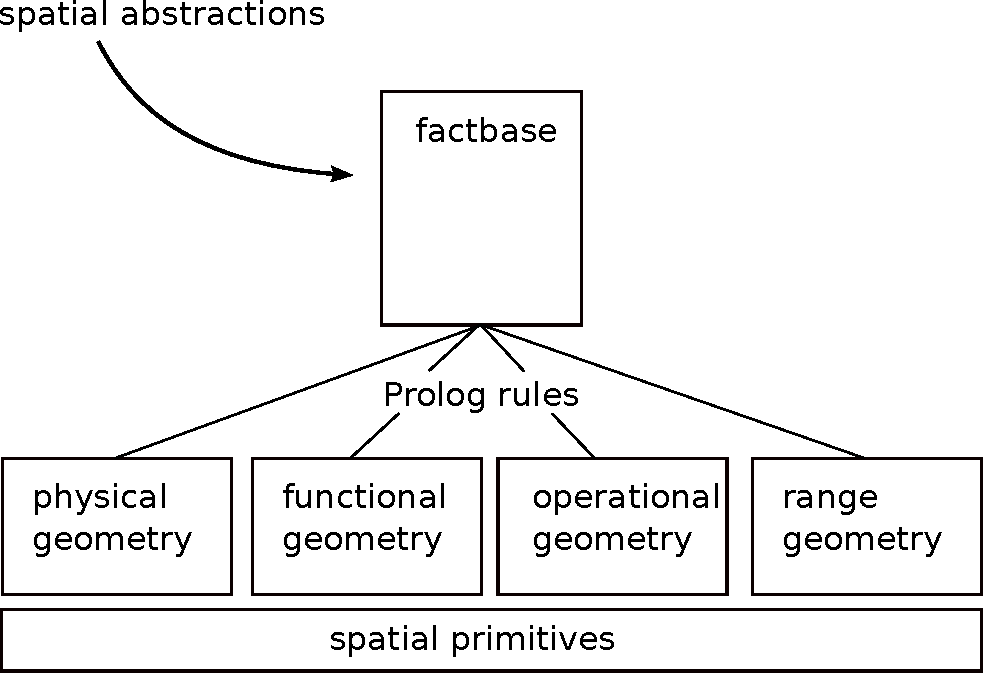
\includegraphics[width=120mm]{clp-design}
\caption{Representation Queries}
\label{clp-design}
\end{figure}

Rulebases link architectural entities to their physical and artefactual representations. There is a separate rulebase for the physical, functional, operational, and range representations that are implemented using a similar form. Each rulebase is built as a series of Prolog rules. The head of each rule links an architectural entity to a variable that is bound to its spatial representation. The body of each rule is responsible for handling coordinate point data by internally defining spatial primitives of points, lines, and polygons. The $spatial \mathunderscore primitive$ rule transforms coordinate data into spatial primitives and binds a variable to a spatial representation. The $spatial \mathunderscore primitive$ rule works by matching arguments. For example, the following call to the $spatial \mathunderscore primitive$ rule with a single point in the second argument instantiates the the variable, \emph{SpatialPrimitive}, as a point object primitive.
\begin{verbatim}
   spatial_primitive(SpatialPrimitive, (5,7)).
\end{verbatim} Similarly, a call to $spatial \mathunderscore primitive$ with a list of points instantiates the variable as a polygon object primitive.
\begin{verbatim}
   spatial_primitive(SpatialPrimitive, [(5,7), (5,9), (7,7)]).
\end{verbatim} 

The following rules show the physical, functional and operational rules for a door with a \emph{crr\_id} of door42. Note the similarities and differences between rules.
\begin{verbatim}
    physical_representation(door42, Geometry) :-
            spatial_primitive(Geometry, [(1,3),(1,4),(4,4),(4,3)]).
            
    functional_representation(door42, FuncGeometry) :-
            spatial_primitive(FuncGeometry, [(1,7),(4,7),(1,1),(4,1)]).
            
    operational_representation(door42, OpGeometry) :-
            spatial_primitive(OpGeometry, [(1,4),(4,6),(4,3)]).
\end{verbatim} Every architectural entity has a physical representation but may or may not have a functional, operational, or range representation. For example, a doorway usually has a functional and operational representation but may not have a range representation. Some entities, such as columns, have no artefactual representations. However, there are no limitation imposed on which entities can or can not have certain artefactual extensions.


These factbases and rulebases can be queried using a Prolog interpretor to retrieve information about architectural entities. A call to the $architectural \mathunderscore type$ factbase can be used to get an entity's type given its' \emph{crr\_id}, such as the following query.
\begin{verbatim}
    architectural_type(door42, Type).
\end{verbatim} The return of this call instantiates the \emph{Type} variable with the door's type, which is \emph{door}. Similarly, a query to a rulebase will return and instantiated variable with the respective spatial representations. Figure \ref{clp-design} shows the implementation structure for querying the rulebases. For example, the following query to the \emph{physical\_representation} rulebase will instantiate the $Geometry$ variable with door42's physical representation. \begin{verbatim}
    physical_representation(door42, Geometry).
\end{verbatim} Calls to the functional, operational, and range rulebases work in the exact same fashion.




%Given an entity and its \emph{crr\_id}, a query to the DSpace rulebase will return an instantiated variable with the entity's quantitative geometry.  
%If the following query is made, the quantitative geometry of \emph{window445} will be instantiated in the \emph{Geometry} variable.

%Within the DSpace CLP framework, the quantitative geometry is defined by geometric primitives of polygons, lines, and points. These primitives are defined by Prolog rules that consume quantitative point data and return an instantiated spatial primitive. The following Prolog rules shows an example of a quantitative rule definition for an entity with \emph{crr\_id window445}. This rule will be stored in the DSpace rulebase. 

%Within the DSpace CLP framework, artefactual geometries are defined using the same spatial primitives as the quantitative geometries. The main difference between the two is that there are multiple rules, one for each artefactual type: functional, operational, and range. An entity may have zero or more artefactual geometries. For example, a doorway in general has a functional and operational representation but does not have one for range representation, while a column has no artefactual representations. The following Prolog rules show and example of a rule definition for the functional and operational representations for a doorway with \emph{crr\_id} of \emph{door55}. 

%Given an entity and its crr\_id, a query to the DSpace rulebase will return an instantiated variable with the entity’s artefactual geometry. Which geometry is returned is based on the rule that is queried. If the following functional representation query is made, the functional geometry of \emph{door55} will be instantiated in the FuncGeometry variable.
%\begin{verbatim}
 %  functional_geometry(door55, FuncGeometry).
%\end{verbatim}

%the multiple perspective model is implemented as a set of Prolog rules. These rules bind architectural entities, via their DSpace identifier (\emph{crr\_id}), to their physical and functional representations. Combining these rules for each entity creates a rulebase that stores each representation in the DSpace CLP framework. This rulebase can be queried to retrieve a specific geometric representation given a \emph{crr\_id}. Figure \ref{clp-design} shows the implementation design for the multiple representation structure in the DSpace CLP framework. Notice that all rules are accessed via the factbase, which stores \emph{crr\_id}'s and ensures that an entity exists before the rulebase is queried. Additionally, all representations are defined over the same set of spatial primitives. This uniformity will be an important aspect of the spatial reasoner in the next section. 


\section{Spatial Reasoning}
Qualitative spatial representation and reasoning is used in the CRR as a link between a design's high level conceptual aspects and its quantitative spatial representations. This process begins by spatially abstracting the design's quantitative spatial representation into spatially abstract objects that are used by the spatial constraint solvers to qualify topological, orientational, and distance relationship over the design, as is illustrated in Figure \ref{quality-quantity-space}. 

\begin{figure}[H]
\centering
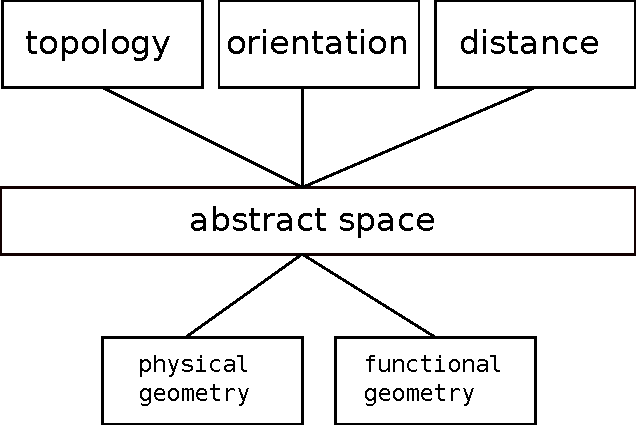
\includegraphics[width=110mm]{reasoner-design}
\caption{Quality \& Quantity Space}
\label{quality-quantity-space}
\end{figure}

These spatial constraint solvers use formal qualitative spatial calculi for topological (RCC), orientational (SCC, OPRA) and distance to qualitatively represent and reason over a design. Within the CLP framework of the CRR, the spatial constraint solvers are implemented using CLP($\mathbb{R}$) (CLP over Reals) and Constrain Handling Rules (CHR). The topological and distance constraint solvers extend Sindalog \cite{Almendros-Jimenez}, a spatial constraint solver written in CHR.

Each spatial constraint solver is implemented as a query engine that qualifies spatial relationships to answer qualitative spatial queries.  A qualitative spatial query involves three step:
\begin{enumerate}
\item retrieval of quantitative representation 
\item spatial abstraction of quantitative representation
\item qualification of spatial relationships
\end{enumerate}  
As an example, the following topological query involves the inside relationship between a desk and a room. 
\begin{verbatim}
   ?- inside(desk3, room1).
\end{verbatim} In step one, the quantitative geometries of the desk and room are retrieved from the physical representation rulebase. The second step uses transformation rules (this will be discussed in the next section) to spatially abstract the physical representation into abstract spatial objects. In the final step, the abstract objects are used by the topological constraint solver to qualify the inside relationship. The constraint solver will respond \emph{true} if the desk has an inside spatial relationship with the room, and \emph{fail} if it does not.   

%The spatial constraint solvers work directly over the design representation structure via the spatial abstraction representation layer and the design factbase. The main service of the reasoner is qualification of the quantitative architectural space into the qualitative feature space of topology, orientation, and distance. It should be noted that the distance constraint solver is different from the topological and orientational constraint solvers because it does not qualify distance relationships, rather it solves minimum distance constraints over quantitative objects. The topological and distance constraint solvers extend The Sindalog spatial constraint solver \cite{Sindalong}, a spatial constraint solver written in CHR. These qualitative spatial relationships are, in turn, used to reason about conceptual design requirements.

The remainder of this section is structured as follow. The first subsection looks at how the quantitative representations are spatially abstracted. The second, third and forth subsections look at topological, orientational and distance based reasoning.

\subsection{Spatial Abstraction}
Spatial abstraction is the process of generalizing a spatial representation so as to represent only those features that are necessary for solving a specific problem. Within the context of the CRR, quantitative spatial representations can be abstracted to points, directed points and convex hulls in order to reason about the design's qualitative spatial relationships of topology, orientation and distance. For example, one approach to reasoning about the qualitative orientational relationship between two doors requires that both doors are spatially represented as directed points. Because doors are naturally represented as polygons, spatial abstraction is needed to transform their quantitative polygonal representation into a qualitative directed point representation.

%In DSpace architectural entities can be spatially abstracted. This allows DSpace to reason about a design from a qualitative level of abstraction with regards to its spatial characteristics of topology, orientation and distance. This type of qualitative spatial reasoning reasons over the abstract feature space of the design using abstract spatial objects of points, directed points, and convex hulls. 

%Architectural entities are not directly modeled as abstract spatial objects. These objects are generated by transformation rules that abstract the quantitative geometries of the architectural entities. 

The process of spatially abstracting an architectural entity depends on the following:
\begin{enumerate} \label{abs dependencies}
\item the type of spatial transformation, eg. line to point, polygon to convex hull
\item the interpretation of the intrinsic nature of an entity within an architectural and design context
\end{enumerate}
For example, the abstracted representation of a doorway as a directed point is not only defined by its physical form (a polygon) but also by the interpretation of the doorway's intrinsic direction in the context of its situation in the design. Further discussion on this topic can be found in \ref{spatial abstraction}.

Within the CLP framework of the CRR, architectural entities are spatial abstracted using Prolog rules. These rules transform an entity's quantitative spatial representation into abstracted objects of points, directed points and convex hulls. Transformation rules take an \emph{crr\_id}, retrieve the quantitative geometry and preform a series of geometric transformations based on the dependencies discussed earlier. For example, the rule to spatially abstract a door into a point involves first retrieves the door's physical representation and then transforming the door's polygonal representation into a point by calculating the polygons centroid. 
\begin{verbatim}
    point_abstraction(Id, PtAbs) :-
           physical_representation(Id, Polygon),
           centroid(Polygon, PtAbs).
\end{verbatim} Given a crr\_id, a query to an abstraction rule will return an instantiated variable with the entity's spatially abstracted geometry. For example, in the following query the point abstraction for door55 is bound to the PtAbs variable.
\begin{verbatim}
    point_abstraction(door55, PtAbs).
\end{verbatim}

%Spatially abstracting an architectural entity depends on the entity type, the spatial abstraction type (point, directed point, or convex hull) and sometimes a contextual identifier (direction of a doorway into or out of a specific room). Given these dependencies, spatially abstraction rules geometrically transform the quantitative geometries into abstract spatial objects. 

%Unlike the quantitative and functional representations, the abstract representation is not stored in the rulebase. Rather, spatial abstraction rules function over the quantitative and functional rulebase. For example, the spatial abstraction rule for a doorway into a point abstraction requires the point abstraction rule to query the quantitative rulebase to retrieve the doorways quantitative geometry. The following spatial abstraction rule is for a doorway point abstraction. Note that the rule is based on the interpretation of a doorway point abstraction as the centroid of its quantitative geometry (see Appendix A.1).   



\subsection{Topology}
The CRR can qualify four topological relationships for convex hulls: inside (\ref{inside}), outside (\ref{outside}), partially overlapping (\ref{overlapping}), and disconnected (\ref{disconnected}). 

\begin{figure}[b]
 \centering
 \subfloat[inside]{\label{inside}
\includegraphics[width=27mm]{ntpp}}
 \hspace{4 mm}
 \subfloat[outside]{\label{outside}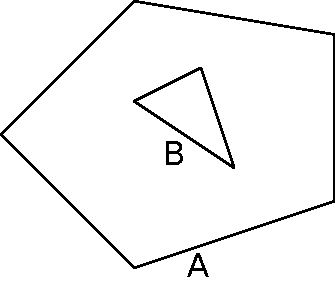
\includegraphics[width=27mm]{ntppi}}
  \hspace{4 mm}
 \subfloat[overlapping]{\label{overlapping}
\includegraphics[width=34mm]{overlapping}}
 \hspace{2 mm}
 \subfloat[disconnected]{\label{disconnected}
\includegraphics[width=43mm]{disconnected}}
 \caption{Topological Relationships}
\label{topoloy}
\end{figure}

An object \emph{A} has an inside relationship with an object \emph{B} if all \emph{A}'s points are inside the convex hull of \emph{B}. The inside relationship is qualified by checking the property of convex hull to point containment. A point in \emph{A} is contained inside the convex hull of \emph{B} if the polarity of the determinate between a point in \emph{A} and each line segment in \emph{B} is negative \cite{compgeom:2000}. In the CRR, points in a convex hull are always ordered counterclockwise, therefore the polarity of the determinant between a point inside the convex hull will always be negative. 

An object \emph{A} has an outside relationship with an object \emph{B} if all \emph{B}'s points are inside the convex hull of \emph{A}. Because the outside relationship is the inverse of the inside relation it is easy to qualify by using the inverse of the inside relationship ($inside(B,A)$). 

An object \emph{A} has a partially overlapping relationship with an object \emph{B} if one or more line segments in \emph{A} intersect with one or more line segments in \emph{B}. The partially overlapping relationship is qualified by checking for line segment intersection between objects. Two objects are partially overlapping if they intersect in at least one point.  

An object \emph{A} has a disconnected relationship with an object \emph{B} if \emph{A} does not intersect with \emph{B}, there are no points in \emph{A} that are inside \emph{B}, and there are no points in \emph{B} that are inside \emph{A}. The disconnected relationship is qualified by checking for line segment intersection and convex hull to point containment. If there are no line segment intersections and no convex hull to point containment relationships, then two objects are disconnected.  

\subsubsection{Spatial Constraint Solver: Topology}
The topological constraint solver qualifies topological relationships over convex hull objects. Its implementation extends the Sindalog \cite{Almendros-Jimenez} spatial constraint solver by integrating topological constraints over convex hulls. It is written using CHR that simplify and propagate topological constraints into geometric constraints of line segment intersection and convex hull to point containment. For example, qualification for the partially overlapping topological relationship involves solving line segment intersection constraints between two convex hulls. The partially overlapping relationship is solved to true when there is at least one line intersection between the convex hulls and it fails when there are none. 

%requires simplifying the overlapping constraint into line segment intersection constraints between the line segments of the convex hulls. The overlapping constraint is solved when at least one line intersection constraint is solved to true or when there are no more line intersection constraints left in the constraint store. In the former case the constraint returns true and in the latter case returns a failure. 

%Once a constraint is in a solvable form, in this case a line intersection or convex hull to point containment constraint, it is solved and returns true or false based on the outcome of the solution. The topological constraint solver is based on successively breaking down a spatial object (convex hull) or spatial primitive (line, point) until solvable geometric constraints can be checked.

The implementation of the partially overlapping relationship begins with a top level constraint that recursively propagates line segment intersection constraints between each line segment in one of the convex hulls. In the following constraint the first argument represents a line segment (two points) and the second is a convex hull (list of points)
\begin{verbatim}
   intersect_segment_hull((Pt1, Pt2), [Pt3, Pt4|PS]) <=>
           intersection_segment_segment((Pt1, Pt2), (Pt3, Pt4)),
           intersection_segment_hull((Pt1, Pt2), [Pt4|PS]).
\end{verbatim} The \emph{intersection\_segement\_segmenet} constraint represents the intersection between two line segments and is in a solvable form. The \emph{intersect\_segment\_hull} constraint is a recursive call that will propagate the \emph{intersection\_segement\_segmenet} constraint for the rest of the convex hull. The qualification for the other topological relationships is similar to the partially overlapping constraint presented here, but in addition to the line intersection constraint some relationships use the geometric properties of convex hull to point containment.

%into the constraint store and will be solved when all points in its arguments are fully instantiated. 

%breaks down a convex hull into its line segments and propagates new constraints for line segment to convex hull intersection. The line segment to convex hull intersection constraint further propagates new constraints that check for line segment to line segment intersection. These constraints are the lowest level constraints and are solved when fully instantiated. The following code shows a propagation rule for the overlapping topological relationship for line segment to convex hull intersection. Line segments are represented as a tuple of point, and convex hull are represented as a list of points.   

The topological constraint solver is used in the CRR to query topological relationships over a design. Given two \emph{crr\_id}'s any of the four topological queries can be made: 
\begin{verbatim}
    ?- inside(Id1, Id2).
    ?- outside(Id1, Id2).
    ?- partially_overlapping(Id1, Id2).
    ?- disconnected(Id1, Id2).
\end{verbatim}Because the topological constraint solver does not know anything about architectural entities there is an intermediate layer between a topological spatial query and the topological constraint solver that is responsible for retrieving quantitative geometries and transforming them into convex hull abstractions. The following rule handles queries for the inside topological relationship.
\begin{verbatim}
    inside(Id1, Id2) :-
            convexhull_abstraction(Id1, Convex1),
            convexhull_abstraction(Id2, Convex2),
            insdie_convexhull(Convex1, Convex2).
\end{verbatim}

%The CRR design representation structure can be queried for topological relationships using the topological constraint solver. Prolog rules query the abstract representation layer to retrieve the spatial abstractions need for topological qualification. In this case objects will be spatially abstracted into convex hulls. The following rule shows the rule for the inside topological relationship. Note that the rule takes two \emph{crr\_id} as arguements, queries the abstract representation layer to retrieve the entities convex hull abstract representations, and then makes a finally call to the \emph{inside\_convexhull} constraint.


\subsection{Orientation} \label{orientation}
The CRR can qualify two types of orientational relationships, intrinsic and extrinsic. Intrinsic orientational reasoning is based on the OPRA$_{m}$ calculus. OPRA$_{m}$ partitions space into half-planes, which are defined by lines emanating from a reference point, and defines the qualitative orientational relationships by the half plane in which a second point is located in relation to the reference point. The granularity of an OPRA$_{m}$ relationship, specified by $m$, defines the number of lines emanating from the reference point. 

\begin{figure}[H]
\centering

\includegraphics[width=60mm]{facing-opra-base-rel}
\caption{OPRA$_{2}$ Space Partitioning}
\label{facing-opra-base-rel}
\end{figure}

Figure \ref{facing-opra-base-rel} shows the OPRA$_{2}$ (two lines) partitioning of space, with labels for the base OPRA$_{2}$ relationships. Point \emph{A} is located in half-plane 7 of point \emph{B}'s partitioned space, and \emph{B} is located in half-plane 1 of \emph{A}'s partitioned space. Note that the arrow depicts the point's direction and the half-planes are labeled starting at the point's direction, incrementing counter-clockwise. 

OPRA$_{m}$ relationships are qualified in the CRR by solving a system of linear inequalities, which are based on the lines that emanate from the reference point. Given a point \emph{A} and \emph{B}, the $\theta_{AB}$ symbol refers to $ \tan^{-1} \frac{B_{y} - A_{y}}{B_{x} - A_{X}} $, the $\phi_{A}$ symbol refers to the direction of point \emph{A}, and the \emph{m} symbol refers to the granularity of the OPRA$_{m}$ relations. Equation \ref{opra-eq} shows the system of linear inequalities that qualify OPRA$_{m}$ relationships as referenced from point \emph{A} to point \emph{B}. Using this system of linear inequalities, the OPRA$_{m}$ relationship ($i$) can be solved for \emph{B} in terms of \emph{A}'s OPRA$_{m}$ space.

\begin{equation}\label{opra-eq}
\begin{aligned}
\Big(&\Big(\Big(\frac{i}{2} \, \in \, N \wedge i < 2\Big) \wedge \Big(2\pi - \frac{i-2}{4m} < \theta_{AB} - \phi_{A} < \frac{2\pi}{4m}\Big)\Big) \\
\lor \;\; \Big(&\Big(\frac{i+1}{2} \in N \wedge i \geq 1\Big) \wedge \Big(\theta_{AB} - \phi_{A} = 2\pi \frac{i-1}{4m}\Big)\Big)\Big) \\ \\
\end{aligned}
\end{equation}

Extrinsic orientational reasoning is based on the SCC. The SCC defines the orientation of a point C (referent) with respect to a point B (relatum) from the viewpoint of a point A (origin).

\begin{figure}[H]
\centering
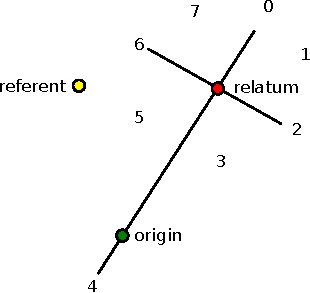
\includegraphics[width=60mm]{scc}
\caption{SCC Partitioning}
\label{scc-partitioning}
\end{figure}

Figure \ref{scc-partitioning} shows an SCC relationship between three points. The partitioning scheme is based on the orientation of the origin and relatum points. In this example, the third point, the referent, is located in half-plane 5 of the SCC partitioned space, so it has an SCC$_{5}$ relationship with point \emph{A} as related by \emph{B}. 

\begin{equation}\label{scc-eq} 
\begin{aligned}
\Big(&\Big(\Big(A_{y} < B_{y}\Big) \wedge \Big(C_{y} > M_{perp} \cdot C_{x} + Y_{perp}\Big)\Big) \; \lor \\
\Big(&\Big(A_{y} > B_{y}\Big) \wedge \Big(C_{y} < M_{perp} \cdot C_{x} + B_{perp}\Big)\Big)\Big) \\
\wedge \;\; \Big(&\Big(\Big(A_{x} < B_{x}\Big) \wedge \Big(C_{y} < M_{AB} \cdot C_{x} + B_{AB}\Big)\Big) \; \lor \\
\Big(&\Big(A_{x} > B_{x}\Big) \wedge \Big(C_{y} > M_{AB} \cdot C_{x} + B_{AB}\Big)\Big)\Big) \\
\end{aligned}
\end{equation}

SCC relationships are qualified by solving a system of linear inequalities, which are based on the lines that partition space into the SCC half-planes. Labeling starts at the line that runs between the origin and relatum, starting at zero and incrementing clockwise. Given three points A, B, and C, $M_{AB}$ refers to the slope of line from A to B, $Y_{AB}$ refers to the y-intercept of the line from A to B, $M_{perp}$ refers to the slope of the line that is perpendicular to the line from A to B, and $Y_{perp}$ refers to the y-intercept of the line that is perpendicular to the line from A to B. Given a point \emph{C}, it has an SCC$_{1}$ relationship with points \emph{A} and \emph{B} if the equations in \ref{scc-eq} can be solved. If the equations are not solvable then \emph{C} does not have an SCC$_{1}$ relationship with \emph{A} related to \emph{B}. There are similar systems of inequalities for each of the seven SCC relationships.  


\subsubsection{Spatial Constraint Solver: Orientation}
The orientational constraint solver qualifies OPRA$_{m}$ and SCC relationships over points and directed points. It is written in CLP($\mathbb{R}$) and uses constraints over linear inequalities (Equations \ref{opra-eq}, \ref{scc-eq}) to solve orientational qualification problems. Within the orientational solver there are two modules, one for intrinsic relationships based on OPRA$_{m}$ and one for extrinsic relationships based on SCC.

The OPRA$_{m}$ constraint solver solves extrinsic orientation qualification problems by constraining the linear inequalities in Equation \ref{opra-eq}. Given an origin point \emph{A}, a reference point \emph{B}, and a granularity $m$, the constraint solver will return the OPRA$_{m}$ relationship ($i$) between \emph{A} and \emph{B}. The linear inequalities are constrained as CLP($\mathbb{R}$) constraints and return once all variables in the linear inequalities are instantiated. 

The SCC constraint solver solves intrinsic orientation qualification problems by constraining the linear inequalities in Equation \ref{scc-eq}. Given an origin, a relatum and a referent, the SCC constraint solver will return true or fail based on the resolvability of the linear inequalities. The linear inequalities are constrained as CLP($\mathbb{R}$) constraints and will return true if the linear equalities are solvable and fail if they are not.

The orientational constraint solver is used in the CRR to query orientational relationships over a design. Given two or three \emph{crr\_id}'s the following orientational queries can be made: 
\begin{verbatim}
    ?- scc(crr_id1, crr_id2, crr_id3, base_relation).
    ?- opra(crr_id1, crr_id2, m, i).
\end{verbatim} Because the orientational constraint solver does not know anything about architectural entities there is an intermediate layer between an orientational spatial query and the orientational constraint solver that is responsible for retrieving quantitative geometries and transforming them into point and directed point abstractions. The following rule handles queries for the scc and opra relationships.
\begin{verbatim}
    scc(Id1, Id2, Id3, BR) :-
            point_abstraction(Id1, Pt1),
            point_abstraction(Id2, Pt2),
            point_abstraction(Id3, Pt3),
            scc(Pt1, Pt2, Pt3, BR).

    opra(Id1, Id2, m, i) :-
            directed_point_abstraction(Id1, DPt1),
            directed_point_abstraction(Id2, DPt2),
            opra(DPt1, DPt2, m, i).
\end{verbatim}


%The CRR design representation structure can be queried for orientational relationships using the orientational constraint solver. Prolog rules query the abstract representation layer and retrieve the spatial abstractions need for orientational qualification: point and directed point. The following rule shows the rule for the SCC$)_{1}$ relationship.

%Given three entities with \emph{crr\_id}’s \emph{door45}, \emph{room53}, and \emph{desk2} the following query will return true if the entities have an SCC$_{1}$ relationship and will fail if they do not. In this specific case they do have an SCC$_{1}$ relationship so the query returns true.
%\begin{verbatim}
%    ?- SCC1(door45, room53, desk2).
%    true.
%\end{verbatim}


\subsection{Distance}
The CRR can calculate the minimum euclidean distance between points, lines, and polygons. Given two objects the minimum distance is calculated by 1) finding the closest point in each object to the other object and 2) calculating the minimum euclidean distance between the two points. 

\begin{figure}[H]
\centering
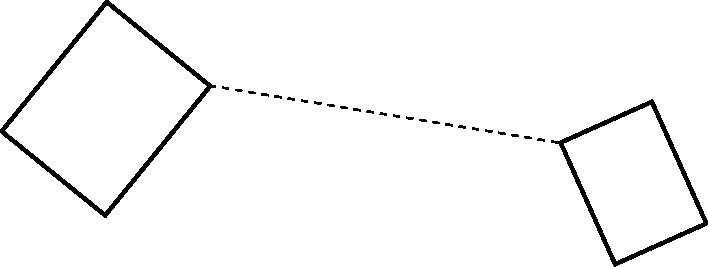
\includegraphics[width=80mm]{min-dist}
\caption{Minimum Distance}
\label{min-dist}
\end{figure}

\subsubsection{Spatial Constraint Solver: Distance}
The distance constraint solver calculates minimum distance queries and uses the distance constraint services of the Sindalog \cite{Almendros-Jimenez} spatial constraint solver for all distance calculations. The distance constraint solver is different from the other two because it returns a specific value, instead of returning \emph{true} or \emph{fail} based on a query. For example, the following query will return the minimum distance between the two objects in D.
\begin{verbatim}
   min_distance(obj1, obj2, D). 
\end{verbatim}

The distance constraint solver is written using CHR that break down the constraints until they can be solved for. This process involves finding the located on each object that is the closest to the other, so that the minimum distance can be calculated between the two. 


\chapter{Design Space} \label{design space}
This Chapter presents the design space module of the CRR. It identifies a set of qualitative spatial attributes found in architecture (QSA) and a set of architectural concepts and show how both can be spatially interpreted using formal qualitative spatial calculi. Additionally, it demonstrates how they can be used to validate conceptual design requirements. 

QSA and architectural concepts were ascertained from literature on architectural design \cite{formfunction} \cite{pattern-language} \cite{Bayazit} and museum research on visitor behavior \cite{Melton} \cite{Bitgood92} \cite{Falk} \cite{Stavroulaki}. Their definitions are explicit characterizations of spatial design concepts that are based on heuristic architectural knowledge and common sense notions of spatial relationships. The objective here is not to be an exhaustive discussion of spatial design concepts or a validation for their spatial interpretation; rather it is to demonstrate how each can be represented and reasoned about in the CRR. 

This Chapter is structured as follows. The first section presents a set of QAS and defines each using formal qualitative spatial calculi. The second section presents a set of architectural concepts that are defined using QSA and spatial relationships. The third section demonstrates how conceptual design requirements can be validated within the framework presented in this Chapter.


\section{Qualitative Spatial Attributes found in Architecture}
This section presents a set of qualitative spatial attributes found in architecture (QSA) and formally defines each QSA using qualitative spatial calculi. QSA are qualities that emerge from a design's spatial characteristics. In general they are defined by the spatial relationships between architectural entities. They can be a perceptual quality that is described from a specific vantage point, or an intrinsic quality that is inherent in the design's spatial structure. 

This section presents five QSA: positioning, positioning for sequences, facing, visibility, and proximity. The goal of this section is to develop a set of QSA that qualitatively describe architectural designs from an experiential perspective. 


\subsection{Positioning}
The positioning attribute defines an orientational relationship between a pair of objects as each object relates to the other within an extrinsic context, i.e., a defined space such as a room, apartment or building. There are four positioning relationships using this scheme: opposing-side of space, same-side of space, left-side of space, and right-side of space. The opposing-side and same-side relationships can be combined, via conjunction, with the left-side or right-side relationships to form the following compound relationships: opposing-left-side, opposing-right-side, same-left-side, same-right-side. Figure \ref{position} shows an illustration of the positioning attribute.

\begin{figure}[t]
\centering
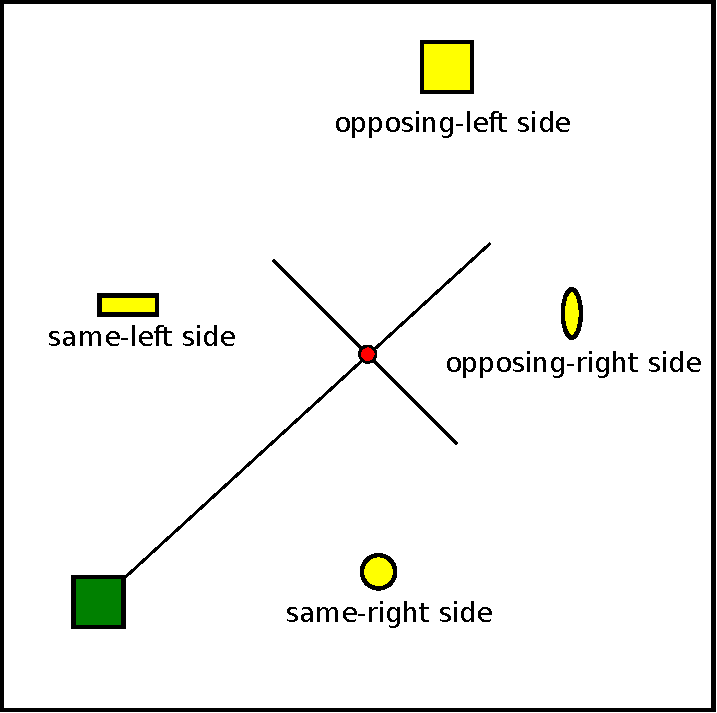
\includegraphics[width=70mm]{position}
\caption{Positioning}
\label{position}
\end{figure}

The positioning attribute is interpreted spatially using the SCC. As discussed earlier, the SCC defines the orientation of a point C (referent) with respect to a point B (relatum) from the viewpoint of a point A (origin). The positioning attribute uses the SCC partitioning scheme to orientationally relate two points (origin, referent) in the context of an external frame of reference (relatum). In the CRR, the reference point is defined as the centroid of the context space. By partitioning space using the centroid, an approximation is made that divides the space into the positioning relationships. An assumption made here is that this space will generally be rectangular in shape.

\begin{figure}[H]
\centering
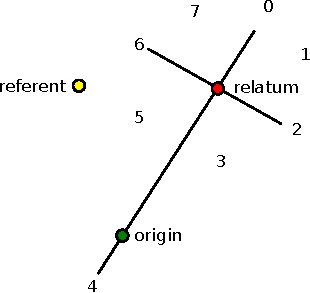
\includegraphics[width=60mm]{scc}
\caption{SCC Partitioning}
\label{scc}
\end{figure}

Using this scheme, two points are defined as being on opposing sides of a space if they have an SCC relationship of 0, 1, 2, 6 or 7, as related by the centroid of the space. Conversely, a pair of points are defined as being on the same side of a space if they have an SCC relationship of 3, 4, or 5, as related by the centroid of the  space. The SCC relationships of 2 and 6 could have been defined for either positioning attribute, the convention here is that they represent an opposing-side relationships. A point is defined as being on the left side of a space from another point if it has an SCC relationship of 5, 6, or 7, and is on the right side if it has an SCC relationship of 0, 1, 2, 3, or 4. Again, the SCC relationships of 0 and 4 could have defined either left or right, the convention here is that they represent the right-side attribute. Using the union set operation these relationships can be combined to form the opposing-left/right, and same-left/right relationships.

These positioning relationships are implemented in the CRR as Prolog rules. There is a single rule for each relationships: opposing-side, same-side, left-side, and right-side. The head of each rule takes three arguments, the first two are crr\_ids for the architectural entities being related and one for the context space. The body of the rule defines the SCC relationships of each positioning quality. The following is Prolog code for opposing-side and same-side positioning rules.
\begin{verbatim}
    opposing_side(Id1, Id2, Id3) :- 
           ( scc(Id1, Id2, Id3, scc0);
             scc(Id1, Id2, Id3, scc1);
             scc(Id1, Id2, Id3, scc2);
             scc(Id1, Id2, Id3, scc6);
             scc(Id1, Id2, Id3, scc7) ).
                                          
    same_side(Id1, Id2, Id3) :- 
           ( scc(Id1, Id2, Id3, scc3);
             scc(Id1, Id2, Id3, scc4);
             scc(Id1, Id2, Id3, scc5) ).
             
    left_side(Id1, Id2, Id3) :- 
           ( scc(Id1, Id2, Id3, scc5);
             scc(Id1, Id2, Id3, scc6);
             scc(Id1, Id2, Id3, scc7) ).
             
    right_side(Id1, Id2, Id3) :- 
           ( scc(Id1, Id2, Id3, scc0);
             scc(Id1, Id2, Id3, scc1);
             scc(Id1, Id2, Id3, scc2);
             scc(Id1, Id2, Id3, scc3);
             scc(Id1, Id2, Id3, scc4); ).                    
\end{verbatim} Conjunction can be used to build the same-left, same-right, opposing-left and opposing-right rules. 
\begin{verbatim}
    opposing_left(Id1, Id2, Id3) :- 
           opposing-side(Id1, Id2, Id3),
           left-side(Id1, Id2, Id3).

    same_right(Id1, Id2, Id3) :- 
           same-side(Id1, Id2, Id3),
           right-side(Id1, Id2, Id3).                                         
\end{verbatim}

The positioning attribute can be used to query if architectural entities or interior design elements are on the opposing or same, left, or right side of a space to the other. For example, a design requirement might state that a bedroom should be positioned to the back of a house from the main entrance. The reason for this requirement is that rooms that are in the back of a house are more private than rooms in the front of the house. In this requirement, the origin is the entrance, the referent is the bedroom, and the relatum is the centroid of the house. Figure \ref{bedroom-positioning} shows a bedroom that is on the opposing side of and apartment from the main entrance. 
\begin{figure}[t]
 \centering
 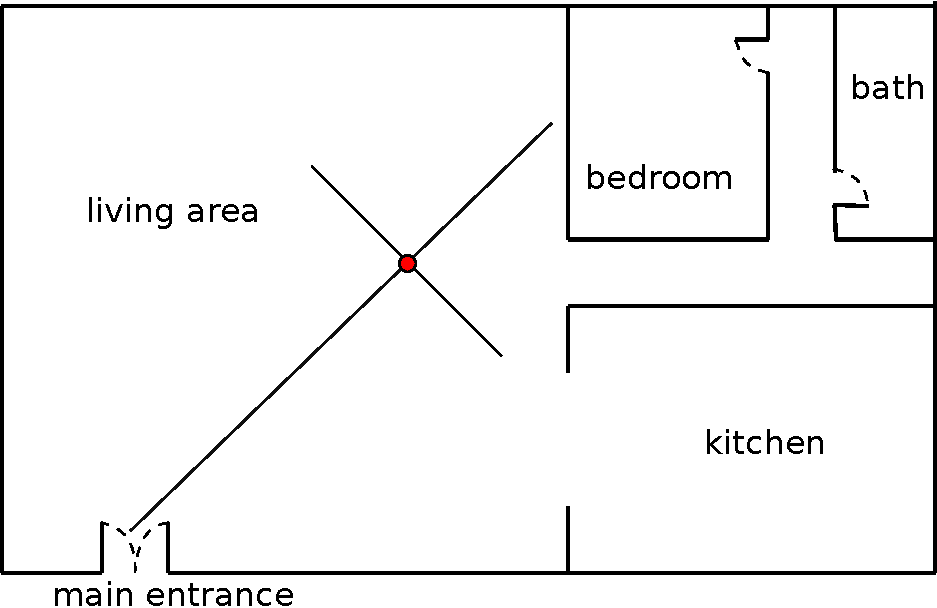
\includegraphics[width=75mm]{bedroom-back-house}
 \caption{Bedroom Positioning}
\label{bedroom-positioning}
\end{figure}



\subsection{Positioning for Sequences}
The positioning for sequences attribute defines a perceptual orientational relationship for a sequence of objects as each relates to a vantage point in an extrinsic context. A sequence is a set of architectural entities, or interior design objects that are grouped together. In general sequences are grouped together based on the proximity (near to each other) but any relationship can define a sequence. There are two positioning relationships for a sequence of objects: horizontal perceived and vertical perceived.  

The positioning for sequence of objects attribute can be spatially interpreted using the SCC. This quality uses the SCC partitioning scheme to orientationally relate a sequence of points (origin, referents) in the context of an external frame of reference (relatum). In the CRR, the reference point is defined as the centroid of the context space. By partitioning space using the centroid, an approximation is made that divides the space into the positioning relationships. As with the positioning attribute, an assumption made here is that the space will generally be rectangular in shape.

Using the SCC partitioning of space, a sequence of objects is perceived horizontally from the vantage point if at least one point in the sequence is on the left-side of the space and at least one point has is on the right. A sequence of points is perceived vertically if they have the following combination of SCC relationships: at least one point in the sequence is on the opposing side of the room and at least one point in the sequence is on the same side of the room. Sequences can be both vertical and horizontal or they can be neither.

Th positioning for a sequence of objects relationships are represented in the CRR as Prolog rules. There is a single rule for each relationship: horizontally perceived and vertically perceived. The head of each rule takes three arguments, the first for the the vantage point, the second is the context space and the third represents the sequence of objects (list of crr\_ids). The following is Prolog code for the horizontal positioning rules. The rule uses two recursive helper predicates (left\_r and right\_r) to iterate through the sequence of objects.
\begin{verbatim}
   horizontally_perceived(Id1, Id2, Seq) :-
           left_r(Id1, Id2, Seq),
           riht_r(Id1, Id2, Seq).
           
   left_r(_, _, []) :- fail, !.           
   
   left_r(Id1, Id2, [Id3, Rest]):-
          ( left_side(Id1, Id2, Id3) -> true ;
            left_r(Id1, Id2, Rest) ).
 	 
   right_r(_, _, []) :- fail, !.           
   
   right_r(Id1, Id2, [Id3, Rest]):-
          ( right_side(Id1, Id2, Id3) -> true ;
            right_r(Id1, Id2, Rest) ).
\end{verbatim}


\subsection{Facing}
The facing attribute defines an intrinsic orientational relationship between two objects as each object relates to the other. The definition used here is based on a common sense interpretation of facing, in which an object \emph{A} is facing towards an object \emph{B}, if \emph{A} is directionally oriented at \emph{B}. Under this definition, a pair of objects can be facing towards or away from each other. Given a pair of objects, \emph{A} and \emph{B}, there are four possible facing configurations between the pair: 

\begin{figure}[H]
 \centering
 \subfloat[A, B towards]{\label{fig:facing-towards}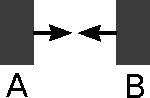
\includegraphics[width=25mm]{facing-towards}}
 \hspace{10 mm}
 \subfloat[A, B away]{\label{fig:facing-away}
\includegraphics[width=28mm]{facing-ABaway}}
  \hspace{10 mm}
 \subfloat[A towards, B away]{\label{fig:facing-A}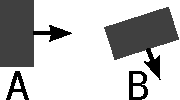
\includegraphics[width=28mm]{facing-Atowards-Baway}}
 \hspace{10 mm}
 \subfloat[A away, B towards]{\label{fig:facing-A}
\includegraphics[width=28mm]{facing-Aaway-Btowards}}
 \caption{facing}
\label{display-arrangement}
\end{figure}

The facing attribute is spatially defined in the CRR using the Oriented Point Relation Algebra (OPRA). The advantage of using OPRA is that it models the intrinsic orientational relationships between a pair of directed points. Using OPRA$_{8}$, the facing attribute can be defined in terms of the half plane sectors. Point \emph{A} is facing towards point \emph{B}, if \emph{B} is located in sectors 0, 1, or 31 of \emph{A}'s OPRA$_{8}$ partitioned space. Similarly, if \emph{A} is located in sectors 0, 1, or 31 of \emph{B}'s OPRA$_{8}$ partitioned space then \emph{B} is facing towards \emph{A}. In this case, both points are facing towards each other. Conversely, point \emph{A} is facing away from point \emph{B} if \emph{B} is located in sectors 2 - 30 of \emph{A's} partitioned space. A granularity of 8 is used in OPRA (i.e., OPRA$_{8}$) to define a narrow interpretation of the facing attribute. 

%Within a room, doorways, windows, and walls are generally face towards each other. By narrowing the space that is considered facing towards, it allows DSpace to detect elements that are more directly facing towards each other.

Figure \ref{fig:facing-opra-towards} shows an example of two points facing towards each other; note that each point is located in sector 31 of the other's partitioned space.  Figure \ref{fig:facing-opra-away} shows an example of two points that are facing away from each other and are not located in sectors 0, 1, 31 of the other's partitioned space. 

\begin{figure}[t]
 \centering
 \fbox{
 \subfloat[facing towards]{\label{fig:facing-opra-towards}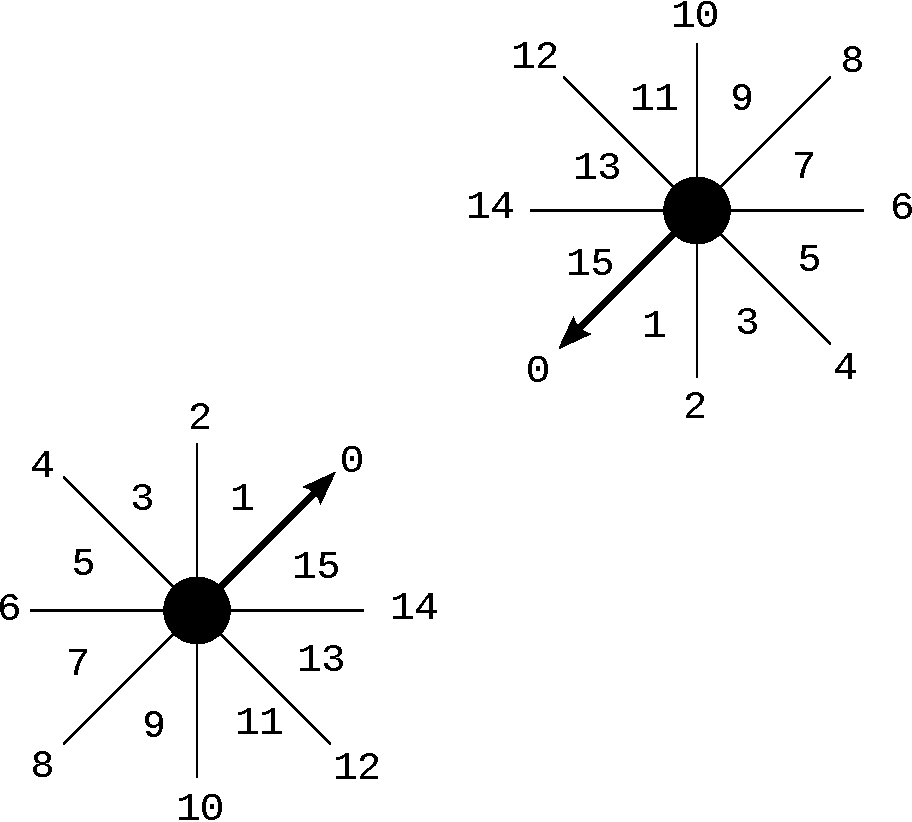
\includegraphics[width=60mm]{facing-opra}}
 }
  \hspace{10 mm}
  \fbox{
 \subfloat[facing away]{\label{fig:facing-opra-away}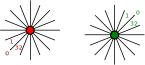
\includegraphics[width=60mm]{facing-away-opra}}
 }
 \caption{OPRA Partitioning }
\label{opra-facing}
\end{figure}

The facing attribute is implemented in the CRR as Prolog rules. There is one rule for facing-towards and one for facing-away. The head of each rule takes two arguments for the architectural entities being related. The body of the rule is a single disjunctive clause that checks for the OPRA$_{8}$ relationship between the architectural entities. Given two architectural objects, the rule returns true if the architectural entities are facing towards or away from each other as defined by the rule, and fails if they are not. The following is Prolog code for the facing rules.

\begin{verbatim}
   facing_towards(Id1, Id2) :- 
          ( opra(Id1, Id2, 8, 0) ;
            opra(Id1, Id2, 8, 1) ;
            opra(Id1, Id2, 8, 31) ).
                                 
   facing_away(Id1, Id2) :- 
          ( facing_towards(Id1, Id2) -> fail; true).                     
\end{verbatim}

In the CRR, the facing attribute can be used to check if two architectural entities or interior design elements are facing towards or away from each other. For example, doorways and windows that face towards each other promote airflow through the space they inhibit. Figure \ref{door-window-facing} shows two example design of a room with a single window and doorway. Figure \ref{fig:door-window-towards} shows the configuration were the doorway and window are facing towards each other, while figure \ref{fig:door-window-away} shows the configuration where the doorway and window are facing away from each other. 

\begin{figure}[h]
 \centering
 \subfloat[facing towards]{\label{fig:door-window-towards}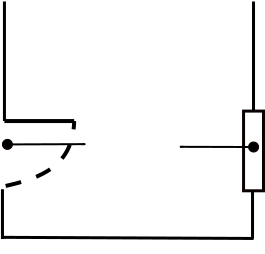
\includegraphics[width=55mm]{door-facing-window-con}}
  \hspace{10 mm}
 \subfloat[facing away]{\label{fig:door-window-away}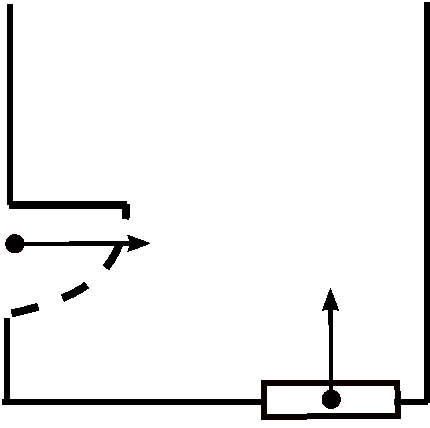
\includegraphics[width=53mm]{door-facing-window-incon}}
 \caption{Door, Window Facing}
\label{door-window-facing}
\end{figure}

%Within the context of architecture, care needs to be taken to account for architectural structures that are long in one axis, such as walls, because the spatial abstraction for OPRA is a directed point. This means that an object is defined as facing towards a wall if it is facing towards the wall's directed point abstraction (usually the centroid of the wall). Under this definition, there are configurations where an object should be considered to be facing a wall but it is not. DSpace handles this special case by modifying the OPRA$_{8}$ relationships that correspond to facing towards and away from a wall. 


\subsection{Proximity}
The proximity attribute defines a qualitative distance relationship between two objects. In the CRR, there are three proximity relationships: near, near+, and far. The spatial interpretation of proximity is defined in the context of architecture, which is restricted here to be \emph{within a building}. Based on this interpretation, proximity is formally defined using heuristics based on what is consider near, near+, and far within a building.   


\begin{figure}[H]
\centering
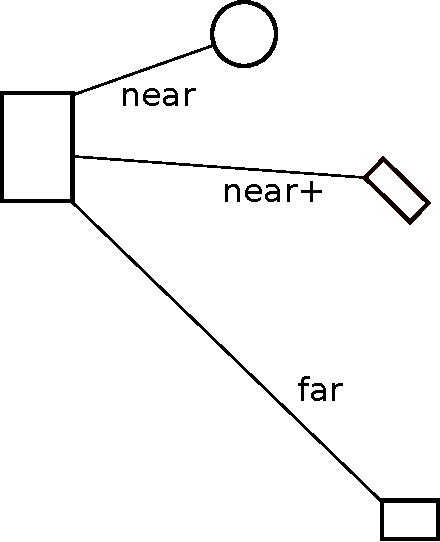
\includegraphics[width=45mm]{proximity}
\caption{Proximity}
\label{proximity}
\end{figure}

Using these heuristics, two objects are near if the minimum distance between them is less then or equal to 6 feet, near+ if the minimum distance between then is between 6 - 12 feet, and far if the minimum distance between them is greater then 12 feet. %While the definition of proximity pivots around 3 and 6 meters, it can easily be changed by using an extra parameter in a proximity predicate. 

Proximity is represented in the CRR as three Prolog rules. There is one rule for near, one for near+, and one for far. The head of each rule takes two arguments for the architectural entities being related. Given two architectural entities, the rule returns true if the objects are near, near+, or far from each other as defined by the rule, and fails if they are not. The following is Prolog code for the proximity rules.

\begin{verbatim}
   near(Id1, Id2) :- 
           minimum_distance_compare(Id1, Id2, <=, 6).
   
   near_plus(Id1, Id2) :-
           minimum_distance_compare(Id1, Id2, <=, 12),
           minimum_distance_compare(Id1, Id2, >, 6).   
   
   far(Id1, Id2) :- 
           minimum_distance_compare(Id1, Id2, >, 12).

\end{verbatim}

The proximity attribute can be used to check whether two architectural entities are near or far. For example, a computer desk should be located near a power outlet to make it easy to power up the desk's computer and desk's lamp. Figure \ref{desk-proximity} shows a desk that is located near a power outlet and another that is not. %Another example is the bathroom should be far away from the kitchen, in order to keep a separation between the two.

\begin{figure}[H]
 \centering
 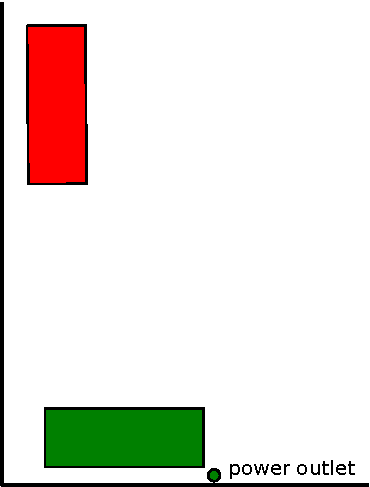
\includegraphics[width=40mm]{desk-proximity}
 \caption{Desk Outlet Proximity}
\label{desk-proximity}
\end{figure}

\subsection{Visibility}
The visibility attribute defines a boolean relationship between a viewpoint and an object with respect to the object being visible from the viewpoint. This interpretation of visibility is based on the topological characteristics of an object blocking (obstructing) a view. It does not take into account the material characteristics of the obstructing object, such as glass, which would allow visibility through the obstructing object. Additionally it does not take into account the effects of distance on visibility, i.e., an object that is very far away is not visible. However, within the context of architecture, the magnitude of distances is limited to a point that it is not a factor in this interpretation of visibility. Under this definition, an objects is visible if the view-space, the space between the viewpoint and the object, is not obstructed.

The spatial interpretation of visibility is based on the topological characteristics of the space in-between the viewpoint and object. This space is referred to as the view-space. An object is visible if the view-space is not obstructed by surrounding structures or objects. An obstructing object is an object that has a partially overlapping or containing topological relationship with the view-space. Artefactual extension is not considered as an obstructing object because it does not have a physical form. This definition does not distinguish between visibility that is partially or totally obstructed.

\begin{figure}[H]
 \centering
 \subfloat[obstructed view]{\label{fig:obstructed-view}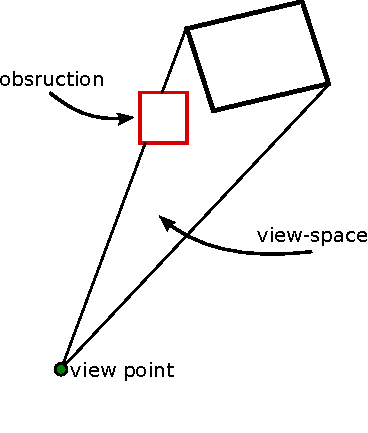
\includegraphics[width=55mm]{visibility}}
  \hspace{10 mm}
 \subfloat[non-obstructed view]{\label{fig:no-obstruction}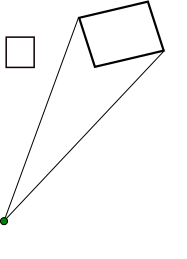
\includegraphics[width=45mm]{visibility-no-obstruction}}
 \caption{Visibility}
\label{Visibility}
\end{figure}

Visibility is represented in the CRR as a single Prolog rule. The head of the rule takes two arguments, the viewpoint and the object that is being check for visibility. The body of the clause calculates the view-space and checks the surrounding objects for a topological obstruction. Surrounding objects are architectural entities that are contained in the same room as the vantage point and object. If the vantage point and object are in different rooms the object is not visible.

Given a viewpoint and an object, the rule returns true if the object is visible, and fails if it is not. The following is the Prolog code for the visibility rule.
\begin{verbatim}
   is_visible(Id1, Id2) :-
           entities_in_same_room(Id1, Id2, Entities), 
           generate_viewspace(Id1, Id2, ViewSpace),
           obstructed_r(ViewSpace, Entities).
           
   obstructed_r(_, []).           
           
   obstructed_r(ViewSpace, [E,Rest]) :-
           disconnected(ViewSpace, E),
           obstructed_r(ViewSpace, Rest).
\end{verbatim} The rule first collects all surrounding objects in the same room as the vantage point and object. It then generates the view-space and then recursively checks for obstructions over the view-space. 

\begin{figure}[h]
\centering
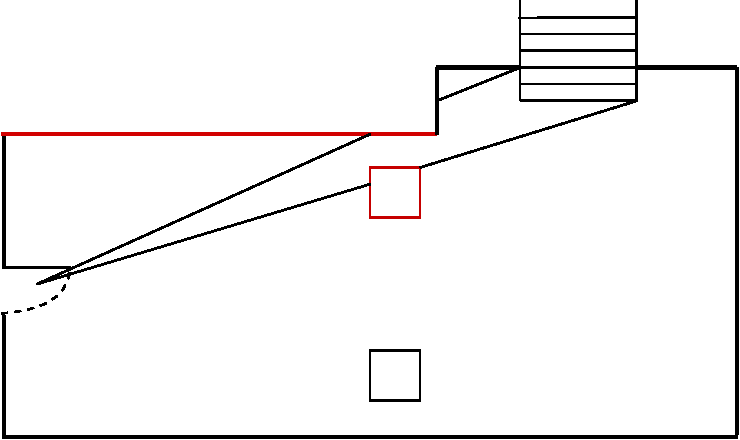
\includegraphics[width=70mm]{visibility-stair-door}
\caption{Visibility Example: Doorway and Stairs}
\label{visibility-door-stair}
\end{figure}

The visibility attribute can be used to check if an architectural structure or interior design element is visible from a given viewpoint. For example, an architect might want to ensure that a staircase is visible from the main entrance of a building, because she doesn't want the staircase to go unnoticed. Figure \ref{visibility-door-stair} shows an example floor plan where the stairway is not visible from the doorway. In this example both the wall in red and column are obstructing the view from the doorway. 




\section{Architectural Concepts}
The architectural concepts of privacy, continuity and enclosure describe experiential aspects of a design \cite{KoileTAC}. These terms are defined in the CRR in a hierarchical manner in which they are built using QSA and qualitative spatial relationships. 

This section presents these three architectural concepts and demonstrates how each is defined in the CRR. Additionally, this Chapter presents characteristics that are influenced by artefactual extension. As in the previous section, the purpose is not to investigate the correctness of the concepts or an attempt to compile a complete list, rather it is to look at how these concepts can be defined logically using architectural qualities and spatial / geometric primitives.

\subsection{Privacy}
In architecture, the concept of privacy implies a notion of separation and obscurity (not being visible). In the case of a room, privacy can be defined as being separated from the main entrance of the building and having doorways that enhances the room's privacy. A doorway can be be defined as private with respect to its functionality of connecting the room to the main area of the house. Under this consideration, a doorway can enhance or hinder the privacy of a room by being visible or not visible from the main entrance.

Within the CRR, the concept of privacy has been formally defined for rooms. A room is private if it has the following attributes: (1) it is positioned on the opposing side of the building with regard to the main entrance and (2) all doorways into the room are not visible from the main entrance.
 
Privacy is represented in the CRR as a Prolog rule. The rule takes a three arguments, which are the room's crr\_id, the entrance's crr\_id and the building's crr\_id. The following is the Prolog rule for privacy. 
\begin{verbatim}
   private(RoomId, EntranceId, BuildingId) :-  
           opposing_side(RoomId, EntranceId, BuildingId),
           get_doors_in_room(RoomId, Doors),
           not_visible_r(EntranceId, Doors). 

   not_visible_r(_,[]).
   
   not_visible_r(Id1, [Id2, Rest]) :-
           not_visible(Id1, Id2),
           not_visible_r(Id1, Rest).   
   
\end{verbatim}

\begin{figure}[b]
 \centering
 \subfloat[Private]{\label{fig:private-room-con}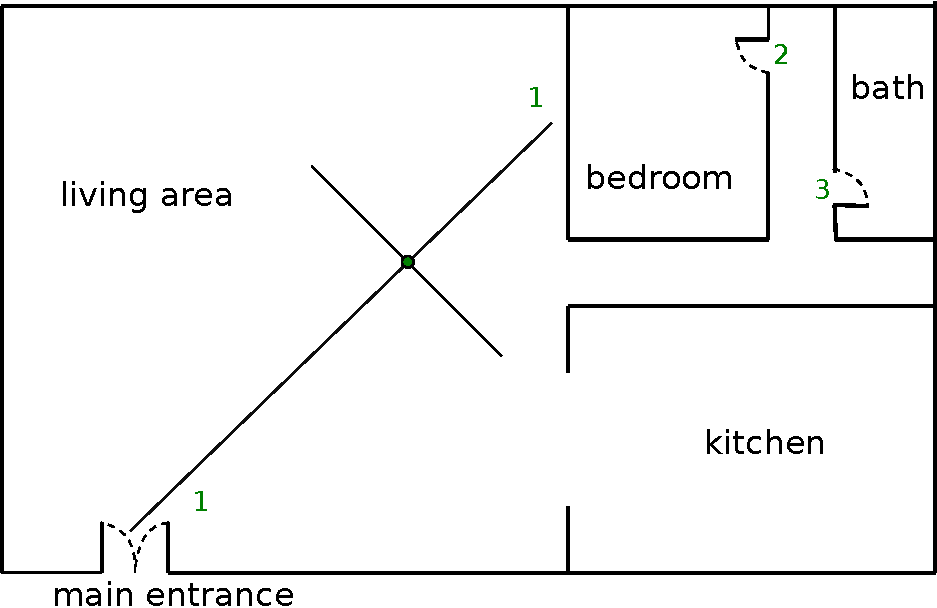
\includegraphics[width=58mm]{privacy-room-con}}
  \hspace{5mm}
 \subfloat[Not Private]{\label{fig:private-room-incon}
\includegraphics[width=58mm]{privacy-room-incon}}
 \caption{Privacy}
\label{privacy}
\end{figure}

Figure \ref{privacy} demonstrates the privacy concept for two floor plans; figure \ref{fig:private-room-con} shows a floor plan with a bedroom that is  private, while figure \ref{fig:private-room-incon} shows a similar floor plan with a bedroom that is not private. The numbers represent the following privacy requirements: (1) the bedroom is positioned on the opposing side of the building with regards to the main entrance, and (2) the doorway is not visible from the main entrance.


\subsection{Continuity}
In architecture, the concept of continuity describes a network of points that are mutually visible \cite{Key}. In the CRR, continuity is interpreted in the context of building navigation and wayfinding and is therefore dependent on continuity between doorways withing the design. Other interpretations of continuity can use any element of the design (beyond doorways), however for the purposes here, continuity only deals with doorways. Under this interpretation a room is continuous if there is continuity between the doorways contained in it. 

Continuity is defined as a network of doorways that are mutually visible. The partitioning of doorways that should be mutually visible is based on a localized containment hierarchy between rooms and doorways, in which doorways that are contained in the same room should maintain continuity. It does not make sense for doorways that are located on opposite sides of a building to be visible to each other, but doorways that are in the same room should be. 

With respect to this definition, continuity is represented as a Prolog rule, which takes a crr\_id for a room, and checks the visibility structures between each doorway located in the room. The following is the Prolog rule for continuity. 

\begin{verbatim}
   continuous(RoomId) :-
           get_doors_in_room(RoomId, Doors),
           mutually_visible_r(Doors).
 
   mutually_visible_r(_, []).

   mutually_visible_r(Id1, [Id2, Rest]):-
           mutually_visible_h(Id1, [Id2, Rest]),
           mutually_visible_r(Id2, Rest).

   mutually_visible_h(_, []).
   
   mutually_visible_h(Id1, [Id2, Rest]) :-
           is_visible(Id1, Id2),
           is_visible(Id2, Id1),
           mutually_visible_h(Id1, Rest).

\end{verbatim}

Figure \ref{continuity} demonstrates the continuity concept for two floor plans. Figure \ref{fig:continuity-con} shows a configuration in which each door is mutually visible to the other doors, and therefore is continuous. Conversely, figure \ref{fig:continuity-incon} shows a configuration in which door1 is not visible to door2 and door1 is not visible door3. The visibility between door1 and door2 is obstructed by a column and the visibility between door1 and door3 is obstructed by a wall. Architectural entities that are red indicated a visibility obstruction. This design is not continuous. 

\begin{figure}[H]
 \centering
 \subfloat[Continuous]{\label{fig:continuity-con}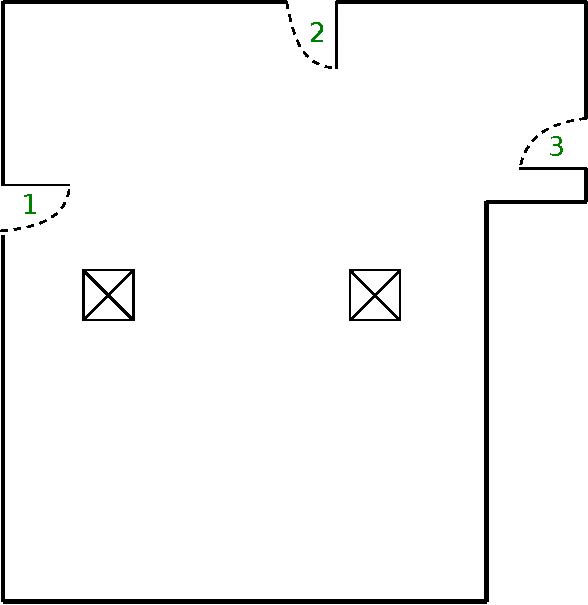
\includegraphics[width=45mm]{continuity-con}}
  \hspace{30 mm}
 \subfloat[Not Continuous]{\label{fig:continuity-incon}\includegraphics[width=45mm]{continuity-incon}}
 \caption{Continuity}
\label{continuity}
\end{figure}

\subsection{Enclosure} 
In architecture, the concept of enclosure defines a space, as experienced from a given vantage point, as being confined or open. In the CRR, enclosure is defined by localized spatial structures in terms of their proximity to a given point. Under this interpretation, a room, apartment, or building can be experienced as both confined and open based on the location of the vantage point within the space. Such a definition takes into account that enclosure is locally experienced. For example, an alcove in an otherwise open room, feels confined when experienced from inside the alcove.

In the CRR, a point is defined as open if less then three walls or columns are near-to the point. Conversely, a point is defined as confined if three or more walls or columns are near-to the point. While this interpretation of enclosure is naive, it maintains the notion that proximity defines the spatial structures of openness and confinement in a localized environment.   

Enclosure is implemented as two Prolog rules, one for confined spaces and one for open spaces. Both rules take a single argument that is a crr\_id for the point being evaluated. The body of each rule calculates the distances characteristics of the local architectural entities to the point being evaluated.
\begin{verbatim}
    confined_space(Id) :-
            room_containment(Id, Rm),
            get_entities_in_room(Rm, Entities),
            num_near(Id, Entities, N),
            N >= 3.            
            
    open_space(Id) :-
            room_containment(Id, Rm),
            get_entities_in_room(Rm, Entities),
            num_near(Id, Entities, N),  
            N < 3.

    num_near(_,[],0).

    num_near(Id1, [Id2|Rest], N) :-
           num_near(Id1, Rest, NRest),
         ( near(Id1, Id2) -> N is NRest + 1 ;
                             N is NRest + 0 ).


\end{verbatim} 

Figure \ref{enclosure} shows a floor plan for a single room with various enclosure properties. The room contains an alcove and a sequence of columns that will provide an environment of confinement. Points in-between the columns and inside the alcove are confined because of the proximity of the walls and/or columns. The points outside of these areas are open because there are few structures nearby.

\begin{figure}[t]
\centering
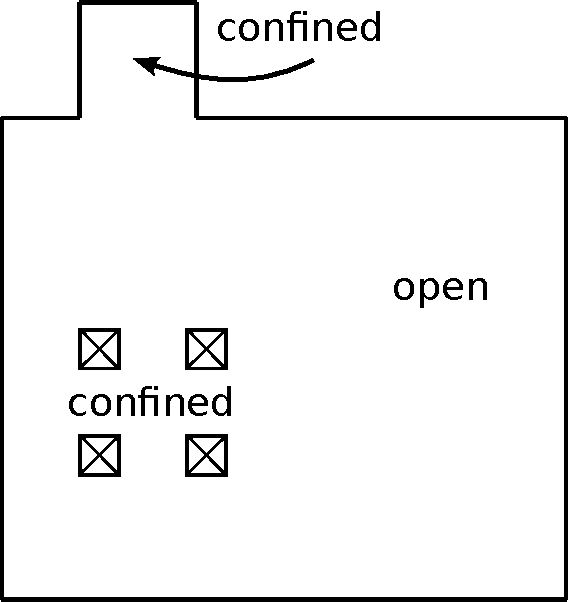
\includegraphics[width=50mm]{spacious-confined}
\caption{Enclosure, Confined and Open}
\label{enclosure}
\end{figure}


\subsection{Artefactual Requirements}
Artefactual requirements are a special case in this section because they are not strictly architectural concepts. However, they provide a unique set of architectural requirements that incorporate a breadth of design aspects. This section will take a look at two examples of artefactual interference. 

Artefactual interference deals with the unintentional interactions of the operational and functional spaces of a building's structural form. For example, the operational space of a bathroom doorway that overlaps with the functional space of the bathroom sink will cause circulation problems into and out of the bathroom. In the CRR, this type of interaction can be detected using topological reasoning over the artefactual extensions of the entities. 

\begin{figure}[H]
\centering
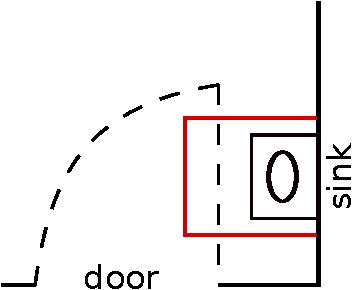
\includegraphics[width=50mm]{door-sink}
\caption{Sink Doorway Interference}
\label{door-sink-example}
\end{figure}

This type of artefactual interaction can be checked for in the CRR using a single rule that takes two arguments in the head of the rule. The body of the rule retrieves the artefactual geometry of each element and checks their topological relationship. It fails if the artefacts have an overlapping relationship.

\begin{verbatim}
   bathroom_sink_door(sink_id, door_id) :- 
           functional_representation(sink_id, SinkFunc),
           operational_representation(door_id, DoorOps),
           not_overlapping(SinkFunc, DoorOps).
\end{verbatim}

Artefactual interactions can be between an architectural entity and artefactual extension. For example, the landing space (i.e., operational space) of a stair should be clear. Representing this requirement is similar to the bathroom sink example except that it checks for interactions between the stair's artefactual space with the building physical space.

In the CRR this can be represented as a single rule. The body of the rule checks for an overlapping relationship between the landing space of the stair and physical structure of surrounding elements.

\begin{verbatim}
    clear_stair_landing(stair_id, physical_id) :- 
            operational_representation(stair, StairOps),
            physical_representation(physical_id, Physical),
            not_overlapping(StairOps, Physical)
\end{verbatim}  

\section{Conceptual Requirement Validation}
The CCR validates design requirements by querying the design's spatial representation using predicate calls to architectural concepts and QSA. Queries will return \emph{true} if the design is consistent, or \emph{fail} if the design is inconsistent per the query. A design is considered consistent if the design's spatial characteristics, as represented in its physical and functional geometries, matches with the definition of the design requirement specification. For example, a design is consistent per a design requirement of a window and doorway facing towards each other, if the spatial characteristic of the design, with regards to the window and doorway, match the spatial specification of facing towards each other. This requirement can be checked for using the following query given a door with crr\_id door543 and a window with crr\_id of window15.
\begin{verbatim}
   ?- facing(door543, window15).
\end{verbatim}
Queries to architectural concepts and QSA can be combined to build requirements. For example, a design requirement for a doorway and window being near to each other can be combined with the previous requirement of facing towards each other to build a new requirement. This requirement can be queried directly or implemented as a new Prolog rule. 
\begin{verbatim}
   ?- facing(door543, window15),
      near(door15, window15).
      
    facing_and_near(Id1, Id1) :-
            near(Id1, Id2),
            facing(Id1, Id2).
\end{verbatim}
Note that the direct query is specific to \emph{door543} and \emph{window15}, while the rule allows the user to input any \emph{crr\_id}'s into the query.
\begin{verbatim}
    ?- facing_and_near(desk52, door6).
\end{verbatim}

Consider the design requirement for a bedroom being private. This requirement can be validated for a design by querying the privacy predicate, as demonstrated above. However, this definition of privacy might not be enough for a particular user. In the CRR, the user can easily extend the definition of privacy by building new Prolog rules that join additional architectural concepts, QSA, and spatial qualities to the existing definition. If the user wants the definition of privacy to include an additional requirement that the bedroom is far away from the living room, the user can construct a new rule by joining the privacy predicate with the proximity predicate. The following is the new predicate for privacy:
\begin{verbatim}
    privacy_new(IdRoom, IdLivingRoom) :-
            privacy(IdRoom),
            far(IdRoom, IdLivingRoom).
\end{verbatim}


%In the CRR CLP framework, QSA and architectural concepts utilize the CRR design representation structure, via the spatial abstraction layer, and the DSpace spatial reasoner to validate conceptual design requirements. QSA and architectural concepts are implemented as Prolog rules. Each rule is implemented as a conjunction of predicates that spatially define the QSA and architectural concepts from a qualitative perspective. Conceptual design requirements can be specified using QSA, architectural concepts, and qualitative spatial relationships. Validating a design requirement happens by making a Prolog query to the CCR that will return \emph{true} if the design is consistent per the requirement or \emph{fail} if the design is inconsistent per the requirement.


\chapter{Museum Case Study} \label{case study}
This chapter presents a case study that demonstrates the application of the CRR in the context of design for an art museum. The purpose is twofold: first, to examine design requirements of an art museum with regards to their affects on visitors experiences in a museum; and second, to demonstrate the application of the CRR for validating these design requirements using a real world museum scenario. 

%how the museum design requirements can be represented and reasoned about in a computational framework, in order to detect design inconsistencies as per the design requirements.

This chapter is divided into two sections. The first section sets up the context of the case study by examining museum design characteristics that influence visitors' behavior and experiences within an art museum. This section has two parts. The first it looks at museum characteristics that affect how visitors behave in museums galleries, and the second part looks at the characteristics of a museum's lobby that influence visitors orientation. The second section of this Chapter demonstrates the CRR by applying the museum requirements to two real world museum designs.  

%examines design requirements in art museums in three parts: the first part looks at requirements that influence museum visitors' behavior. The second part looks at requirements for promoting exploration in the museum. The third part looks at the requirements of accessibility and security within the museum. The second section, looks at how these requirements can be interpreted spatially and represented in the CRR. The third section tests the DSpace reasoner using sample museum floor plans that are both consistent and inconsistent per the design requirements for several art museums. The objective of this demonstration is to show that the DSpace reasoner can validate a design against its design requirements.


\section{Museums}
Museums are a place of public education, in which art, historical artefacts, and scientific exhibits are put on display for the public to view \cite{Falk}. While museums in general have many common threads in terms of their design requirements, this case study takes the approach of narrowing the study to that of an art museum. This focuses the discussion to specific real world examples and maintains the perspective that this is not an exhaustive study of museum design requirements, rather it's an investigation into the nature and interpretation, with respect to the spatial characteristics of a set of design requirements. Additionally, the point is not to prove the validity of these requirements in an empirical sense; rather it is to show the process of representing and reasoning about design requirements in a formal computational framework.

The art museum is a unique and fruitful choice for this case study because it provides a rich set of design properties that have been formally studied and reported \cite{Melton} \cite{Bitgood02} \cite{Falk}. Within museum studies, visitor behaviour has been one of the primary focuses, starting with experiments dating back to the 1930's. 

\subsection{Museum Design Requirements}
Pretend for a moment that you are an architect working on the initial design for a new modern art museum. During your first visit with the museum's curator you discuss several design requirements that are important for the new museum. Your discussion reveals that the curator wants the new art museum to adhere to the following two requirements:

\begin{enumerate}
\item Maximize visitor utilization of exhibitions
\item Maximize visitor orientation in lobby
\end{enumerate}

While these requirements are abstract, they can be mapped to concrete spatial characteristics of museum design. The following section looks at several of these characteristics.


\subsection{Maximizing Visitor Utilization of Exhibitions}
This portion of the case study will look into four factors that influence visitors' movement patters: positioning of doorways, spatial arrangement of display cases, positioning of furniture and statues, congestion, and exploration. These properties inform museum designers about the spatial characteristics that influence the utilization of the museum's exhibitions.


\subsubsection{Positioning of doorways}
In an important study \cite{Melton}, Melton discovered that the most influential factor to determine  the amount of attention an exhibition piece receives is the pieces's position relative to doorways in a gallery room. Prior to this, museum researchers believed that the pieces's intrinsic properties of `interestingness', color, and size were the contributing factors that determined the amount of attention a piece received. Melton explained why this happens; he demonstrated that the amount of attention a piece receives is directly related to the visitor circulation patterns within the museum and these circulation patterns emerge from the spatial characteristics of the museum's architecture.

\begin{figure}[H]
 \centering
 \subfloat[circulation pattern]{\label{fig:door-opposite}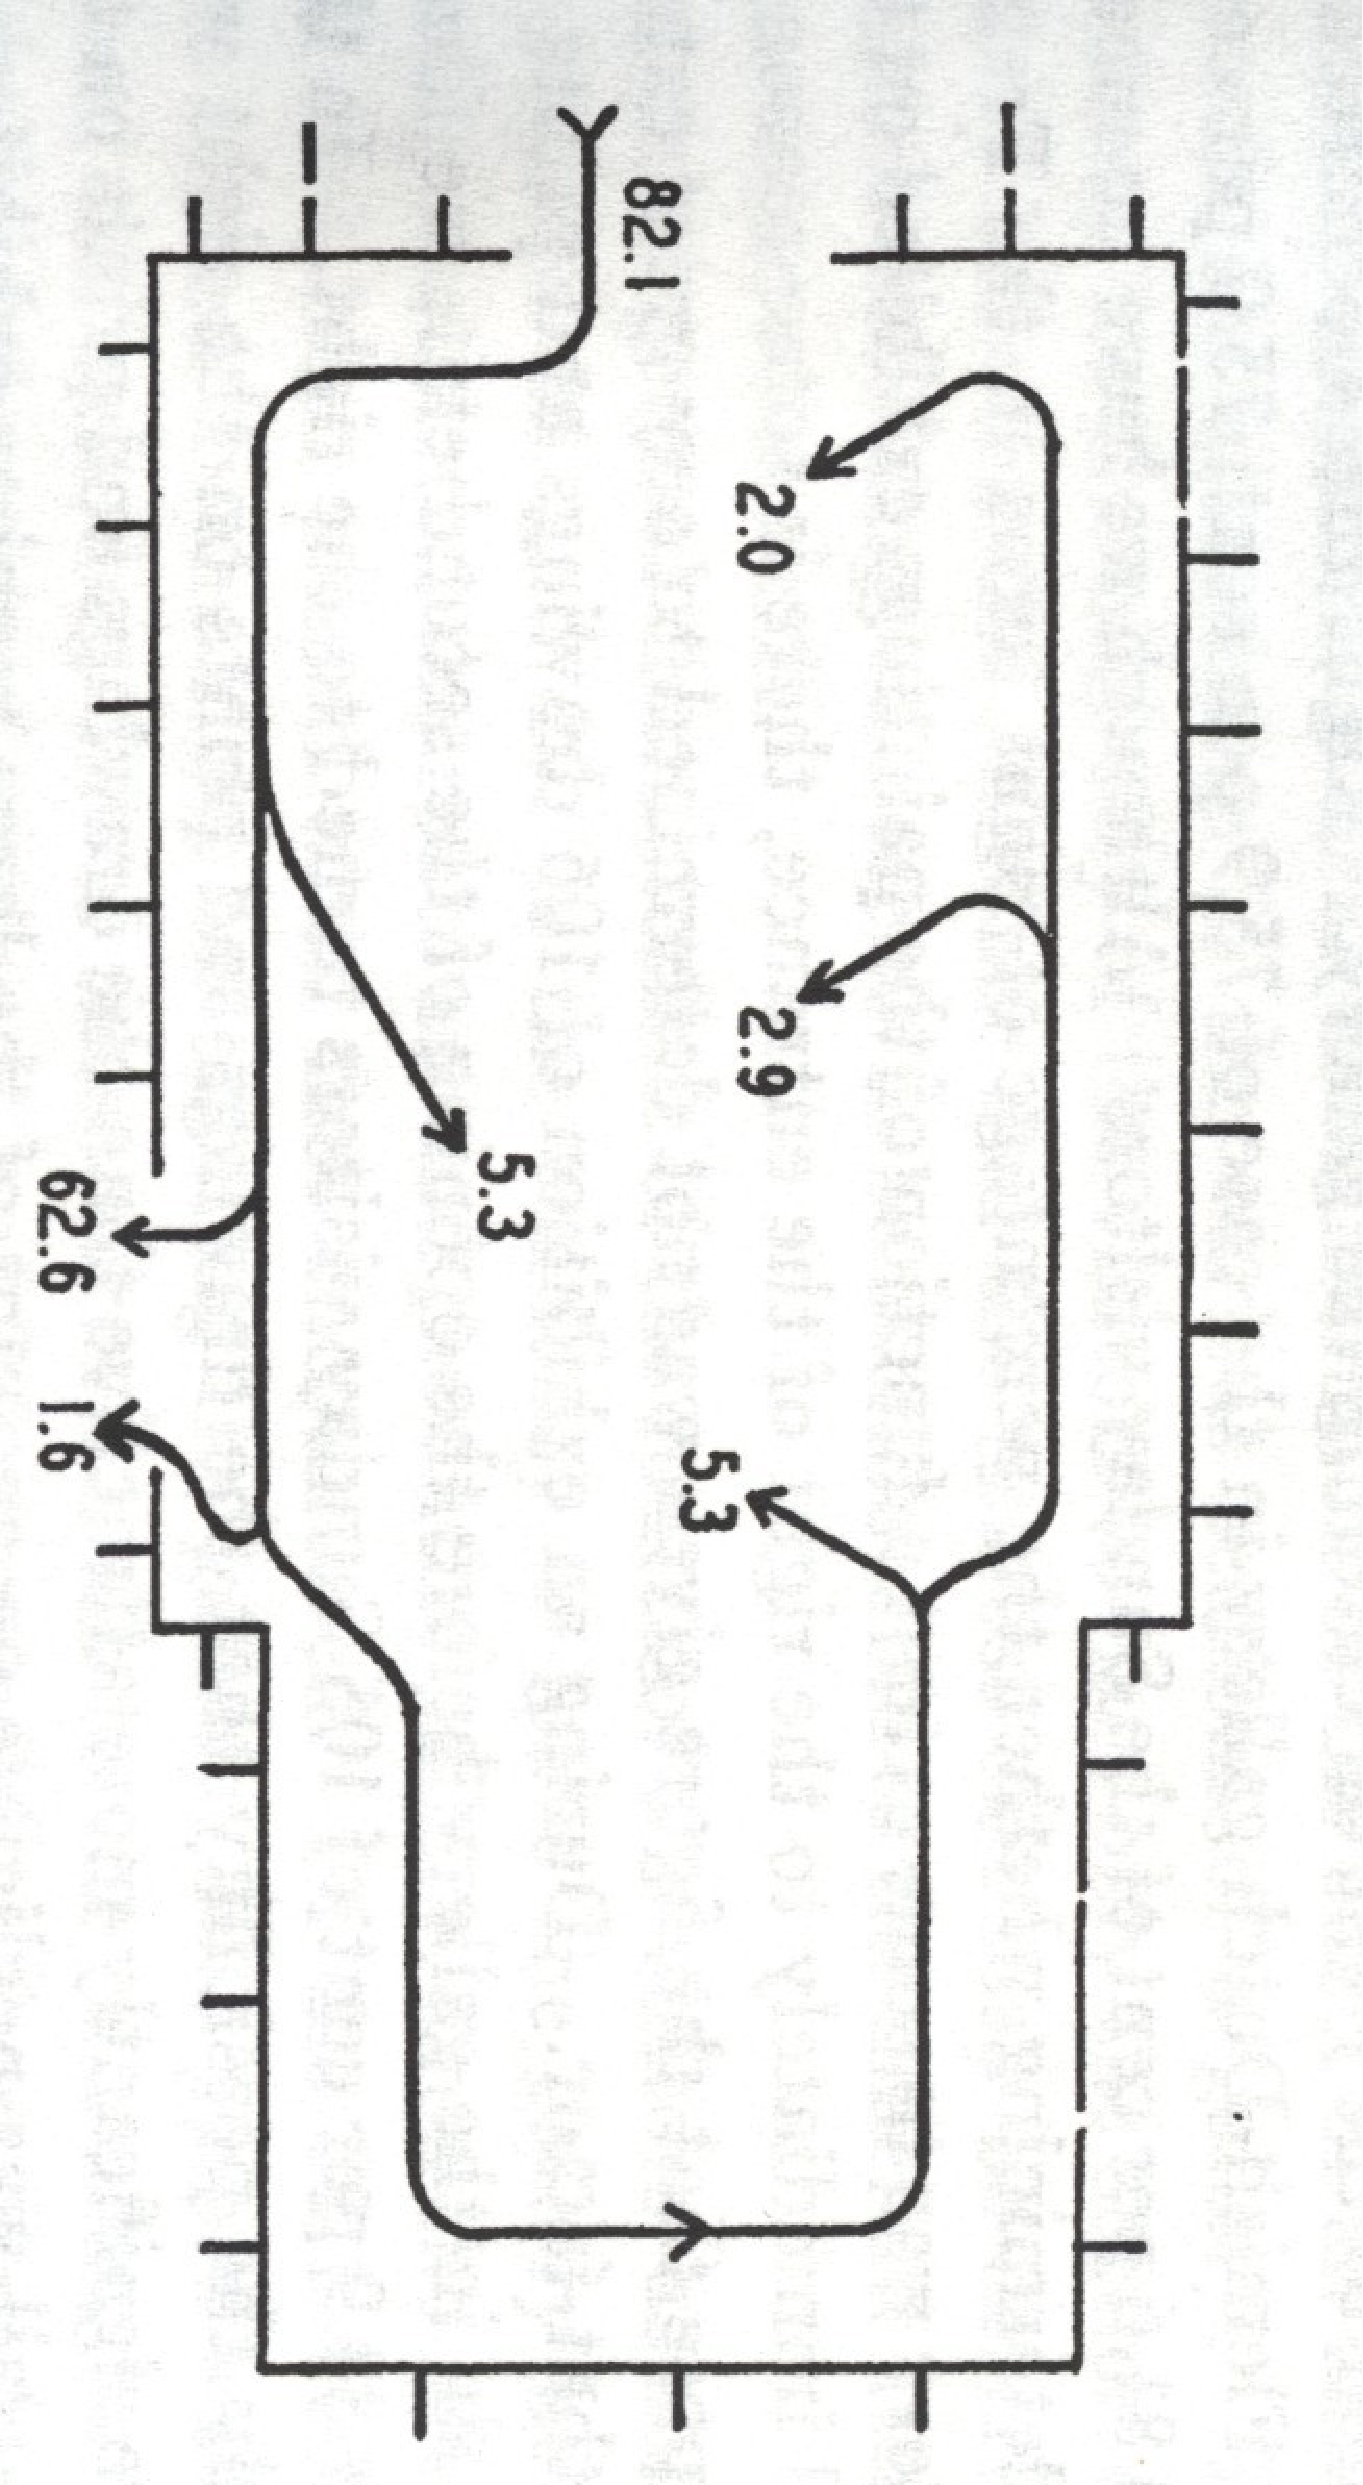
\includegraphics[width=35mm, angle=90]{melton-circulation}}
 \hspace{10 mm}
 \subfloat[frequency of visits]{\label{fig:door-opposite}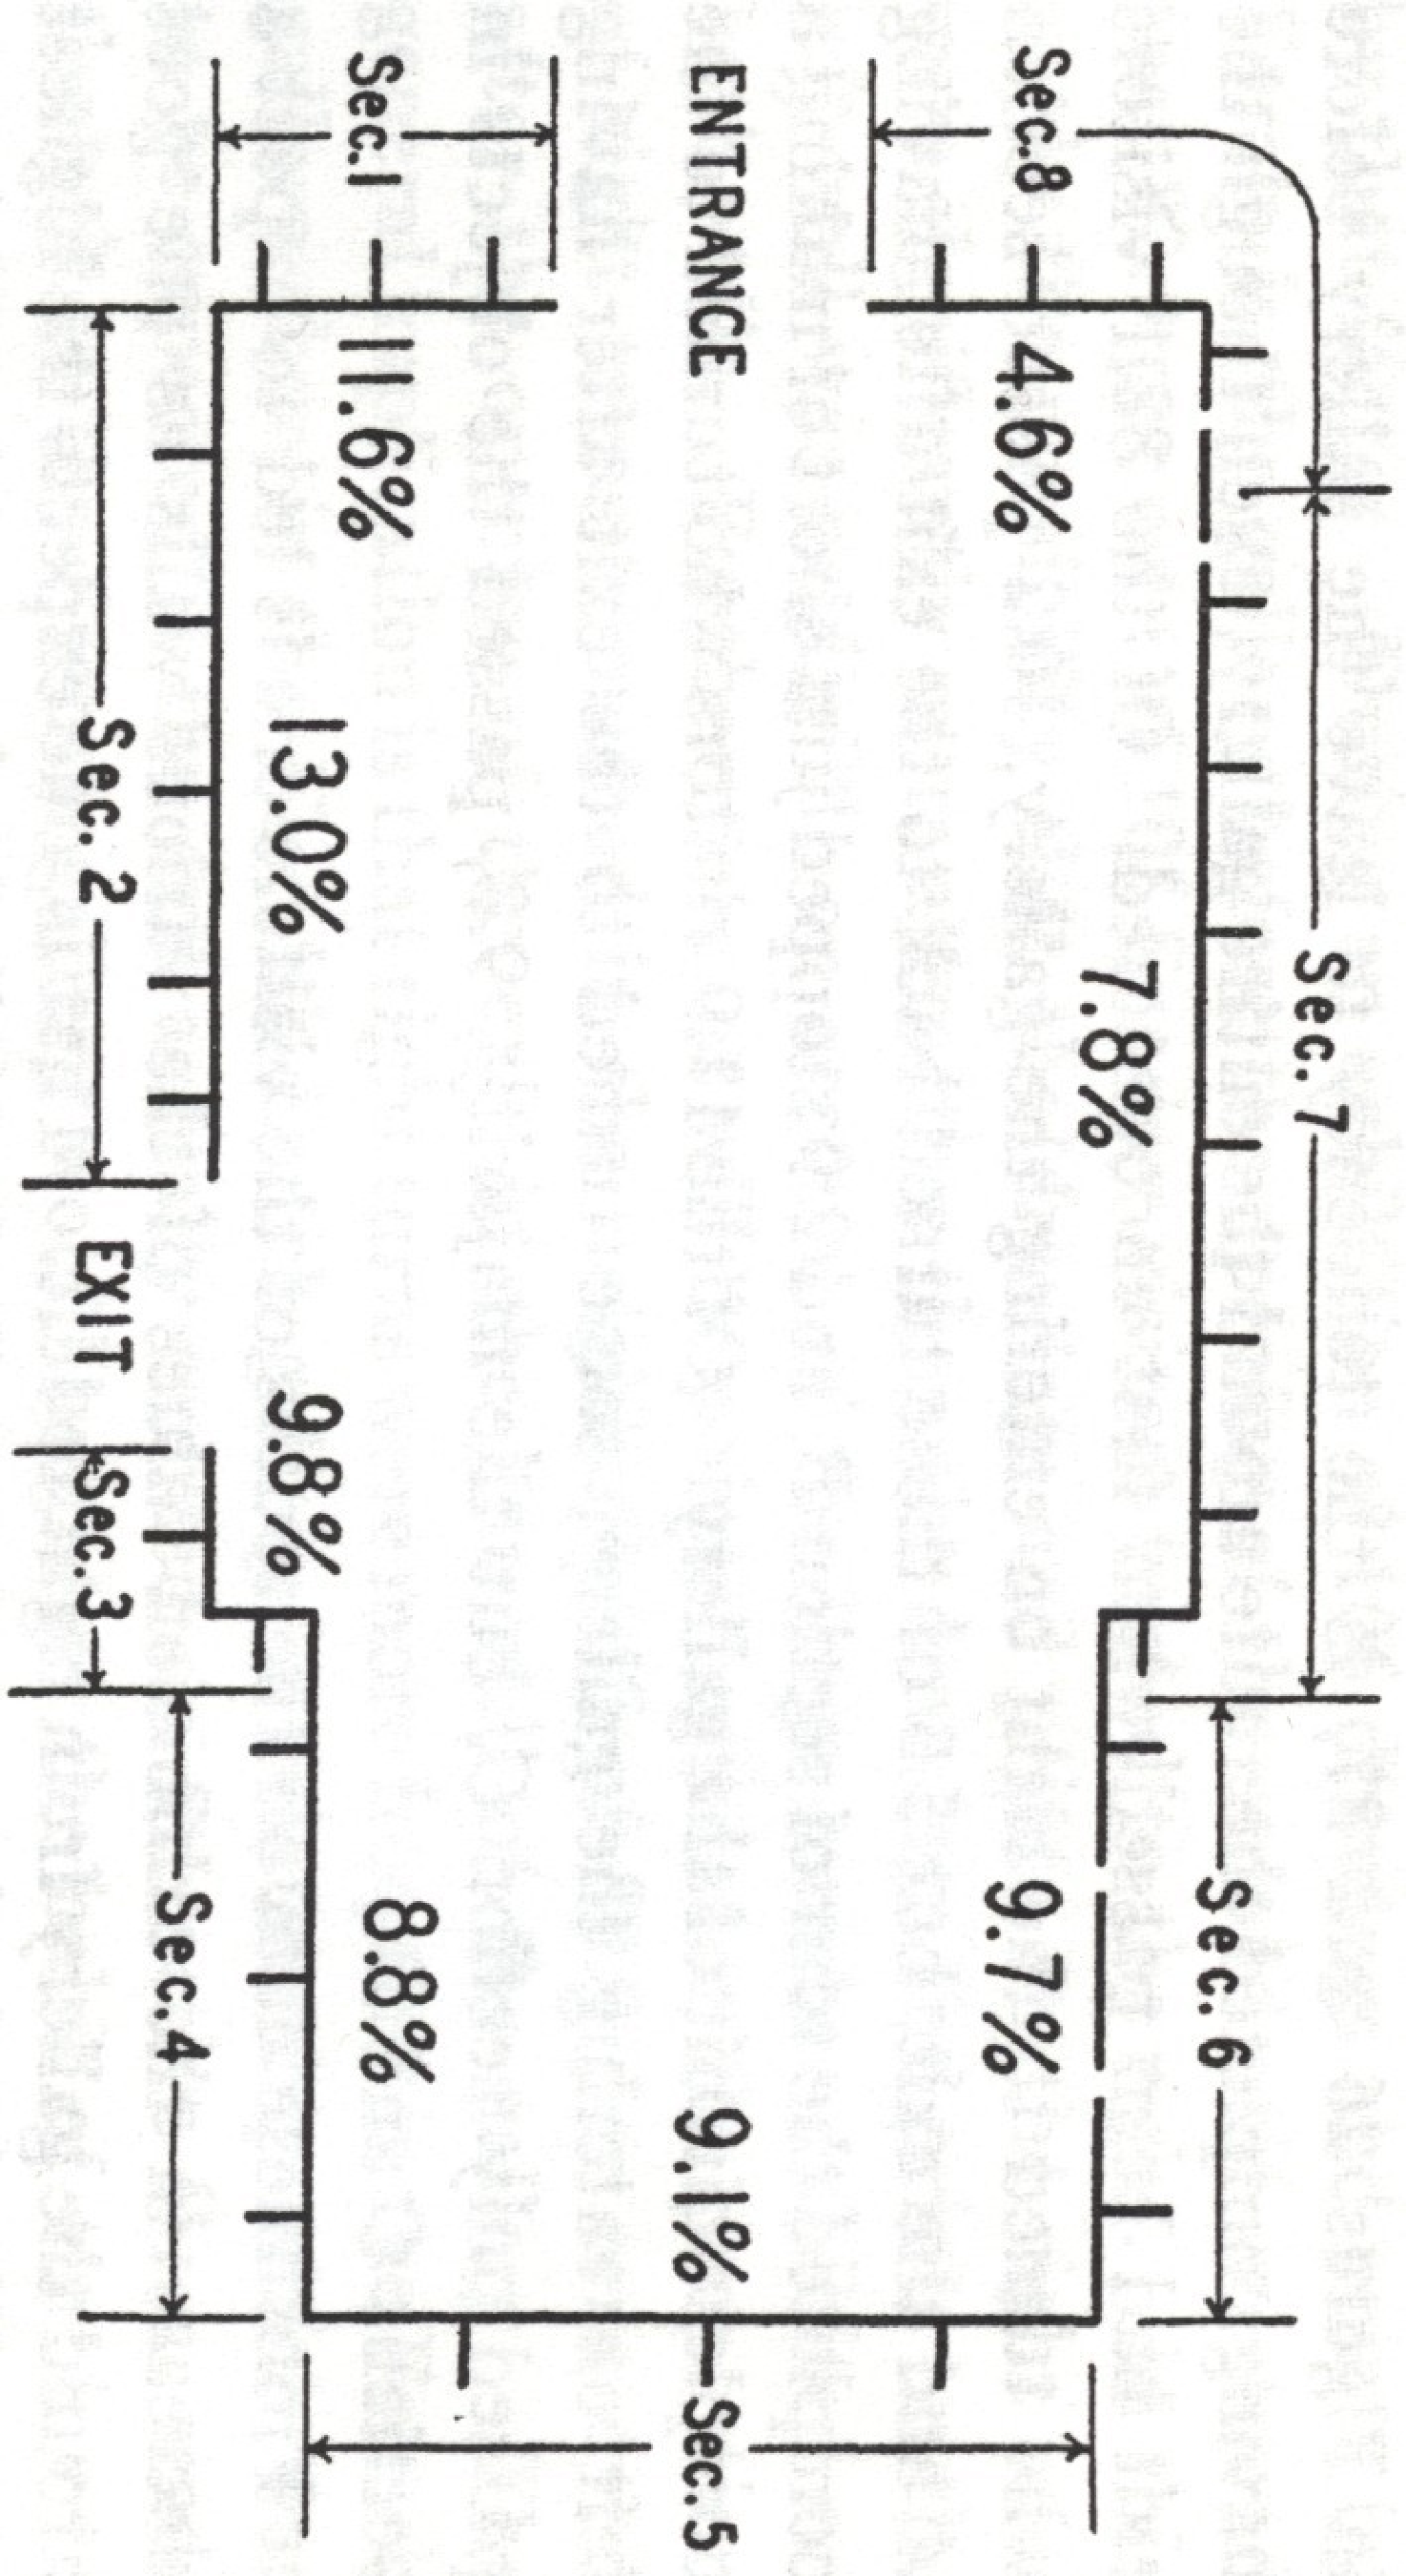
\includegraphics[width=35mm, angle=90]{melton-frequency}}
 \label{melton}
 \caption{Results from Melton's experiments on the effects of door positioning in an Art Museum}
\label{Melton-studies}
\end{figure}

The crux of Melton's experiments suggested that visitors exit through the first door they encounter, which he referred to as the exit gradient. Figure \ref{Melton-studies} shows the results of an extensive study of visitors circulation patterns and stopping frequencies in an art museum. The studies reported that almost 80 percent of visitors exited through the first exit they encountered before viewing the entire exhibition. Additionally, the studied showed that the most frequently visited objects where those located along the shortest path from the entrance to the exit. 

%Furthermore, Bitgood suggests that visitors tend to follow along the wall that is closest to the door they entered \cite{Bitgood95}. Given that visitors also tend to exit through the first doorway they encounter, doorways should not be positioned in a wall that is close to an entrance. 

The results of Melton's studies inform architects of spatial characteristics that influence movement patterns in exhibitions. Specifically, doorways that are positioned on the same side of a gallery room and doorways that are near to each other cause visitors to pay attention to fewer exhibits than doorways that are positioned on opposing sides of a gallery room and doorways that are far away from each other.\footnote[1]{These two requirements pertain to galleries with exactly two doorways. Galleries with more or less doorways have not been studied.}

\begin{description}
\item[Gallery Requirement 1:] \emph{Gallery doorways should be positioned on opposing sides of the gallery room.} 
\item[Gallery Requirement 2:] \emph{Gallery doorways should far away from each other.} 
\end{description}

Figure \ref{museum-doors} shows two gallery exhibition designs. Considering Gallery Requirement 1, Figure \ref{door-positioning-con} shows a design that is consistent with the requirement, while Figure \ref{door-positioning-incon} shows a design that violates the requirement.
\begin{figure}[H]
 \centering
 \subfloat[Opposing Side]{\label{door-positioning-con}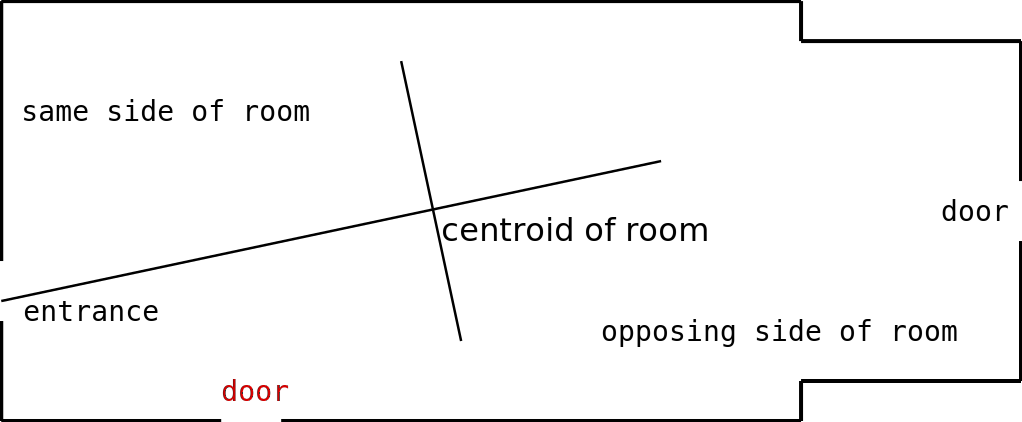
\includegraphics[width=68mm]{door-possitioning}}
 \hspace{6 mm}
 \subfloat[Same Side]{\label{door-positioning-incon}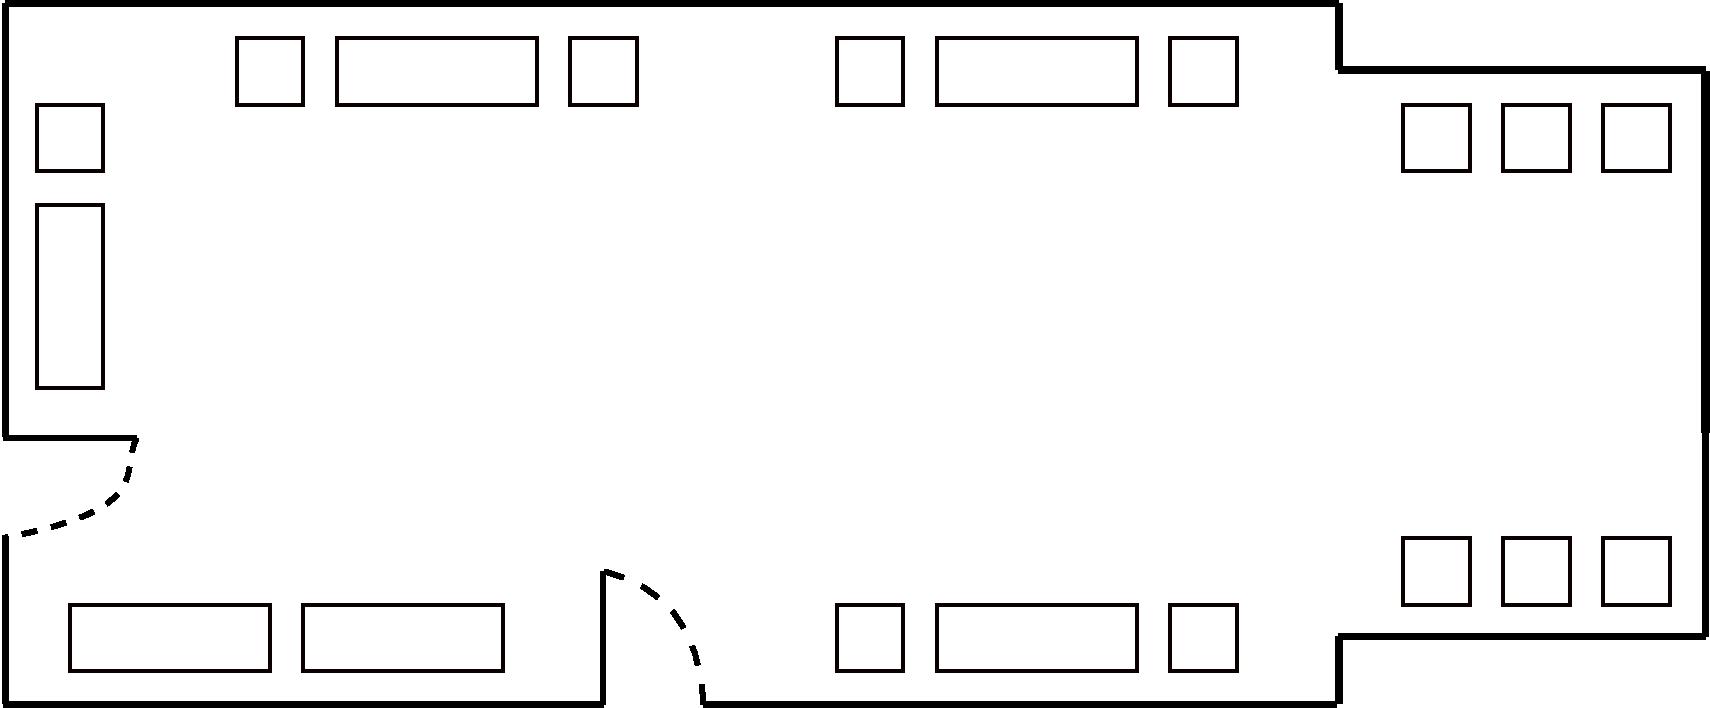
\includegraphics[width=68mm]{door-possitioning-incon}}
 \label{melton}
 \caption{Positioning of Doorways in Galleries}
\label{museum-doors}
\end{figure}


\subsubsection{Placement of display cases}
The placement of display cases in galleries has been shown to influence visitors' movement patterns. Bitgood \cite{Bitgood92} showed in some environments that display cases that are located at the perimeter of a gallery generate the most amount of attention, while display cases that are isolated in the middle of the gallery received the lowest amount of attention.

\begin{figure}[H]
 \centering
 \subfloat[Isolated]{\label{island}
\includegraphics[width=35mm]{island}}
 \hspace{10 mm}
 \subfloat[Perimeter]{\label{perimeter}
\includegraphics[width=35mm]{perimeter}}
 \caption{Display case arrangements}
\label{display-arrangement}
\end{figure}
 
\begin{description}
\item[Gallery Requirement 3:] \emph{Display cases should be located on the perimeter.}
\end{description} 

Figure \ref{display-arrangement} shows two illustrations. Figure \ref{island} show a display case that is an isolated  near the center of the gallery, while Figure \ref{perimeter} shows a display case that is located at the perimeter of the gallery. 

Additionally, the placement of a sequence of display cases can disrupt circulation patterns when the sequence cuts horizontally across the view of a visitor as they are entering the room. This type of display pattern might cut off part of the gallery from the visitors normal visitation patterns by changing circulation pathways.

\begin{description}
\item[Gallery Requirement 4:] \emph{Display cases sequences should not cut horizontally across the view of a visitor located at an entrance.}
\end{description} 

\begin{figure}[H]\label{cut-horizontal}
\centering
\subfloat[Not Horizontal]{\label{not-cut}
\includegraphics[width=65mm]{sequence-no-cut}}
\hspace{10 mm}
\subfloat[Horizontal]{\label{cut}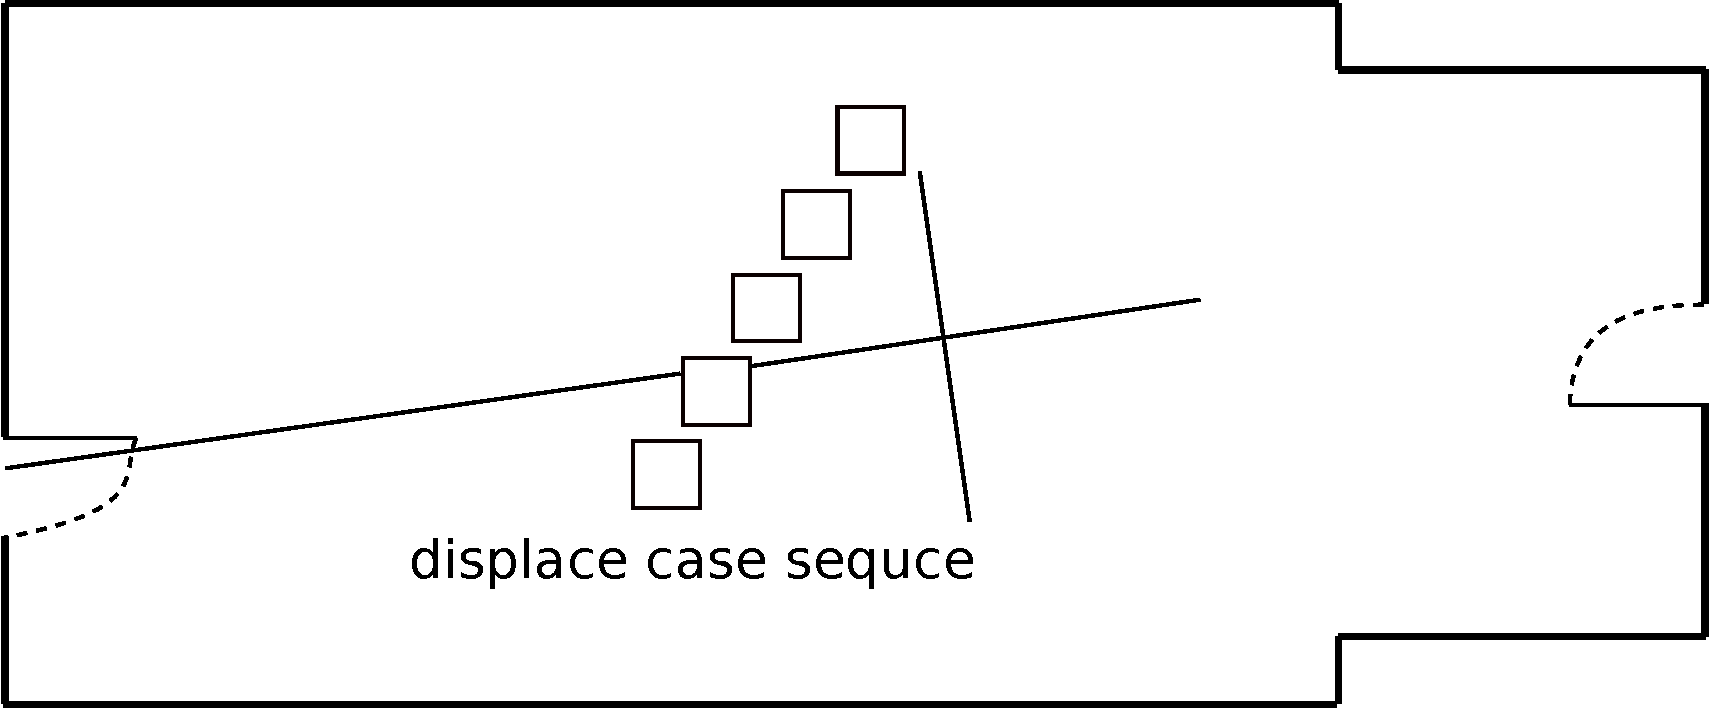
\includegraphics[width=65mm]{sequence-cut}}
\caption{Display Case Sequence}
\end{figure}

Figure \ref{cut-horizontal} shows two example galleries with displace case sequences. Figure \ref{not-cut} shows an example where the display case sequence does not cut horizontally across the visitor's view, while Figure \ref{cut} shows an example where the display cases sequence does cut horizontally.

\subsubsection{Congestion}
Congestion in museums can be caused by artefactual interference between the viewing space of displayed objects with movement pathways of visitors. In order to reduce congestion in museums, designers should be aware of the placement of display cases and furniture (seating benches) within the gallery. The following requirement should be followed to reduce congestion in museums.

\begin{description}
\item[Gallery Requirement 5:] \emph{There should be no artefactual interference between museum display cases, museum seating and architectural entities.}
\end{description}


\subsubsection{Positioning of benches and statues}
The positioning and orientation of benches and statues can increase the amount of attention an exhibition receives and change circulation patterns within a gallery \cite{Stavroulaki} \cite{Museum}. Studies have shown that seating facing a doorway or window will decrease attention in the Gallery.

\begin{description}
\item[Gallery Requirement 6:] \emph{Gallery seating should face away from doorways and windows.}
\end{description}

The orientation of a statue to doorways can increase the attention the statue receives as well as objects close to it. Statues that face away from doorways encourage visitors to move around the statues in order to get a better view.  
\begin{description}
\item[Gallery Requirement 7:] \emph{Statues should face away from doorways.}
\end{description}


\subsubsection{Exploration}
The way visitors explore an exhibition is influenced by the spatial characteristics of the layout, as well as the characteristics of each gallery room. Layouts that are sequential (one way in, one way out), promote a controlled and orderly flow of movement. Museums of history and science are well served by this type of design because they have a narrative to tell that is chronological. On the other hand, layouts that present the visitor with path choices (multiple doorways), promote free-flowing exploration. In this type of layout it is important that visitors are aware of the path choices that are available. This means that doorways are visible between each other throughout the layout. This concept of visibility between a network of points is referred to as continuity and is an important characteristic of layouts that present visitors with multiple path choices.  

\begin{description}
\item[Gallery Requirement 8:] \emph{The layout of the museum should maintain continuity between doorways within each gallery room.}
\end{description}

%Within a Gallery, rooms that are open promote more free-flowing exploration than rooms that are narrow. Narrow rooms inhibit exploration because of space limitations and confinement. Rooms that are open provide more space for visitors to explore the room in a free-flowing manner.
%\begin{description}
%\item[Requirement 11:] Gallery rooms should be open, rather than confined, in order to promote free-flowing exploration.
%\end{description}


\subsection{Visitor Orientation in the lobby}
The lobby is the first place visitors encounter when they enter a museum. The design of the lobby is important because it not only provides a first glimpse of the museum's exhibits but it is the place where the museum provides services to its visitors, including: a ticketing desk, bathrooms, and entrances to exhibitions \cite{Bitgood02}. The aim of the requirements for the lobby focus on making it easy for visitors to locate services and orient themselves to the new environment. 

Upon entering the lobby most visitors need to find the ticket area. It is important, therefore, that the ticketing area is visible from the entrance. Additionally, studies have shown that people first look to their right hand side when entering a building. By placing the ticket area on the right hand side of the lobby, visitors are more likely to notice it immediately upon entering the lobby. Finally, the ticketing area should be close to visitors when they enter because it is likely one of the first places they will need to visit.
\begin{description}
\item[Lobby Requirement 1:] \emph{The ticketing area should be visible from the main entrance.}
\item[Lobby Requirement 2:] \emph{The ticketing area should be on the right hand side of the lobby from the entrance.}
\item[Lobby Requirement 3:] \emph{The ticketing area should be close to the entrance.}
\end{description}

After obtaining a ticket most visitors will try to locate the entrance to the exhibitions. Therefore, exhibition entrances should be visible from the ticketing area to make it easy for visitors to find where they need to go next. 
\begin{description}
\item[Lobby Requirement 4:] \emph{Exhibit entrances should be visible from the ticketing area.}
\end{description}

%Bathrooms are an important services for museum visitors. Surprisingly, the place of the bathroom can have an impact on how long visitors stay in the museum. Studies \cite{tbd} have found that bathrooms that are located on the same side of the lobby as the entrance encourage visitors to leave earlier compared to museums with bathrooms on the opposing side of the lobby from the entrance. 

%\begin{description}
%\item[Lobby Requirement 5:] \emph{The bathroom should be on the opposing side of the lobby from the entrance.}
%\end{description}


\section{Application of CRR for Museum Design}
This section presents the application of the CRR to two real world museums using the gallery and lobby requirements. This section is organized as follows. The first part introduces the two museums that are used in the case study and briefly describes the process of importing them into the CRR from ArchiCAD. The second part presents the results of using the CRR for for validating the museum gallery and lobby requirements to the two museums.

%of applying the CRR to the museums to detect violations with regards to the museum design requirements. 

%for validating art museum design requirements using real world scenarios. The first part of this section introduces the museums that will be used in the case study and gives a brief overview of process of importing them into the CRR. The second part of this section presents the results of applying the museum design requirements identified above to these museums.

%This use case is from the perspective of a museum designer and covers the process of importing a museums design from an architectural design tool (ArchiCAD) into the CRR, the building of museum requirements using architectural concepts and QSA, and finally validation of the requirements using the CRR query engine. 

\subsection{Museum Designs and Import}
This case study uses the Asian Art Wing of the Philadelphia Museum of Art \cite{Philadelphia} and the lobby of the Museu Calouste Gulbenkian \cite{Gulbenkian}. The Asian Wing of the Philadelphia Museum of Art will be used for the demonstration of the gallery requirements, while the lobby of the Museu Calouste Gulbenkian will be used for the demonstration of the lobby requirements. The motivation behind using real world museums instead of contrived examples is to demonstrate the CRR in a real world context with regards to the practicality of museum design requirements.

\begin{figure}[H]
 \centering
 \subfloat[2nd Floor]{\label{art museum}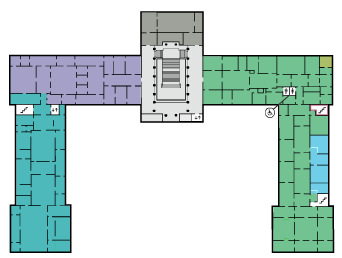
\includegraphics[width=78mm]{philadelphiamuseum}}
 \hspace{10 mm}
 \subfloat[Asian Wing]{\label{asian wing}\includegraphics[width=45mm]{asianwing}}
 \caption{Philadelphia Museum of Art - Source \cite{philadelphiamusem}}
\label{art-museums}
\end{figure}

The Asian Art Wing (gallery rooms 226 and 238-245), shown in Figure \ref{asian wing}, and the lobby of the Museu Calouste Gulbenkian were manually built in ArchiCAD 14. The dimension and scale of the rooms where obtained from the museums to ensure as much accuracy to the real design as possible. Benches, display cases and statues were added to demonstrate some of the museum requirements. Figures \ref{philadelphia-museum-floorplan} and \ref{lobby} show the floor plans for both museums in ArchiCAD.

\pagebreak

\begin{figure}[H]
\centering
\includegraphics[width=120mm]{lobby}
\caption{Lobby of Museu Calouste Gulbenkianin}
\label{lobby}
\end{figure}

\begin{figure}[H]
\centering
\includegraphics[width=90mm]{museum-floor-plan-reqs-p}
\caption{Asian Wing of Philadelphia Museum of Art}
\label{philadelphia-museum-floorplan}
\end{figure}

Once the museums are built in ArchiCAD they are imported into the CRR via a Multi-Modal Spatial Data Access Framework \cite{carl}. This framework provides the CRR with access to various design information, via the Industry Foundation Class data exchange format \cite{IFC}, including: the physical representation for each architectural entity, and room / building / story containment relationships. Artefactual representations, room to wall boundary relationships, and wall to door / window containment relationships are manually added into the CRR. Future versions of the Multi-Modal Spatial Data Access Framework plan on supporting these informational design aspects. The import process consists of a parser written in Python that parses a Design Space schematized xml file, produced by the Multi-Modal Spatial Data Access Framework, and outputs a Prolog representation of the design that is used by the CRR.


\subsection{Validating Museum Requirements}
The results of applying the museum gallery and lobby requirements to the Philadelphia Museum of Art and the Museu Calouste Gulbenkian are presented in Table \ref{results}. This Table contains three columns. The first column identifies the museum requirement, the second column shows the CRR query used to check for the requirement, and the third column show all violations that were discovered by the CRR. The results here demonstrate two outcomes. The application of the gallery requirements to the Philadelphia Art Museum gives an examples of where the design is inconsistent with regards to the requirements, while the application of the lobby requirements to the Museu Calouste Gulbenkia gives an example where the design is consistent with the requirements. 

\begin{table}[t]
  \begin{center}
  \begin{tabular}{ | c | p{7.2cm} | p{7.3cm} |}
    \hline
    Req. & CRR Query & Violations\\ \hline
    GR1 & opposing\_side(\emph{door\_id}, \emph{door\_id}, \emph{room\_id}) & $\circ$ door4, door10, gallery240 
    													\newline $\circ$ door5, door11, gallery243 
    													\newline $\circ$ door7, door12, gallery241 \\ \hline
    GR2 & far(\emph{door\_id}, \emph{door\_id})  &  $\circ$ door4, door10 
                                          \newline  $\circ$ door5, door11
                                          \newline  $\circ$ door7, door12 \\ \hline
    GR3 & near(\emph{display\_id}, \emph{wall\_id}) & $\circ$ display4 \\ \hline
    GR4 & horizontal(\emph{display\_list}) & $\circ$ (display0, display1, display2, display3) \\ \hline
    GR5 & artefact\_interference(\emph{id}, \emph{id}) & $\circ$ door8, display8 \\ \hline
    GR6 & facing\_away(\emph{bench\_id}, \emph{door\_id}) & $\circ$ bench0, door6
                                                   \newline $\circ$ bench1, door3 \\ \hline
    GR7 & facing\_away(\emph{statue\_id}, \emph{door\_id}) & $\circ$ statue0, door6 \\ \hline
    GR8 & continuity(\emph{room\_id}) &  $\circ$ gallery239 \\ \hline
    LR1 & visibility(\emph{entrance\_id}, \emph{desk\_id})& no violations\\ \hline
    LR2 & right\_side(\emph{entrance\_id}, \emph{desk\_id})& no violations \\ \hline
    LR3 & near(\emph{entrance\_id}, \emph{desk\_id})& no violations\\ \hline
    LR4 & visibility(\emph{desk\_id}, \emph{door\_id})& no violations\\
    \hline
  \end{tabular}
  \end{center}
\caption{Case Study Results}
\label{results}
\end{table} 

It should be noted that the quantification of requirements is not handled in this version of the CRR. Therefore, checking requirements may involve several queries or special consideration from the user. For example, Gallery Requirement 6 can be quantified as: for every pairing of benches and doorways within a gallery room, each pairing should be facing away from each other. In this example the user is responsible for checking the facing relationship between each pair of doorways and benches. As another example, Gallery Requirement 4 can be quantified as follows: for every display case there should be at least one wall that is near to it. In this example the user is responsible for checking the proximity relationships between each display case and all walls surrounding it. 

\begin{figure}[t]
\centering
\includegraphics[width=90mm]{coninuity-req-view}
\caption{Visibility in Gallery239}
\label{continuity-gallery239}
\end{figure}

Requirement violations reported in Table \ref{results} can be visually verified by looking at Figure \ref{philadelphia-museum-floorplan}. For example, Gallery Requirement 1, which specifies that doorways should be on opposing sides of a gallery room, can be visually inspected to verify the CRR results. In this example, the CRR reported that the following doorways and gallery rooms are in violations of Gallery Requirement 1:
\begin{itemize}
\item door4, door10, gallery240
\item door5, door11, gallery243
\item door7, door12, gallery241
\end{itemize} Visual inspection of Figure \ref{philadelphia-museum-floorplan} confirms that these doorways are \emph{not} on opposing sides of the gallery room and therefore are in violation of Gallery Requirement 1. As another example, Gallery Requirement 8 specifies that every Gallery should maintain continuity between doorways. The results of this case study shows that gallery 239 is in violation of the requirement. The cause of this violation is because door3 and door10 are not visible from door9, and vice versa. Figure \ref{continuity-gallery239} shows a 3-D view of gallery 239 from the perspective door10 (this graphic was rendered in ArchiCAD) and show that in fact door3 and door10 are not visible from door9 because there is a wall obstructing the view.

\begin{figure}[h]
\centering
\includegraphics[width=90mm]{museum-floor-plan-reqs-crop2}
\caption{Gallery Requirement Violations}
\label{art museum in archiCAD}
\end{figure}

The process of manual verification can be used to inspect the other gallery requirement violations reported by the CRR. The result of doing so will show that the CRR accurately reported violations for this case study. To illustrate this, Figure \ref{art museum in archiCAD} shows the Philadelphia Art Museum floor plan with labels for corresponding gallery requirement violations as reported in Table \ref{results}. 

Similarly, this same process can be used to verify that the lobby of the Museu Calouste Gulbenkian is consistent with the lobby requirements. For example, Lobby Requirement 2 specifies that the ticketing desk should be on the right hand side of the entrance from the perspective of entering the museum. Inspecting figure \ref{lobby} shows that in fact the ticketing desk is on the right hand side. Manual inspection of the other lobby requirements will show that the Museu Calouste Gulbenkian is consistent with the lobby requirements as reported by the CRR.

This case study demonstrated the application of the CRR to reason about conceptual design requirements given an underlying CAAD-based spatial representation of the design. The crux of the work here is the use of a qualitative spatial layer that intermediates between the conceptual level and quantitative level. The results show that the CRR is capable of accurately detecting design requirement violations and informs the designer when a design is consistent of inconsistent per the designs requirements.

%Gallery Requirement 1 specifies that doorways should be positioned on opposing sides of a gallery room. The opposing side relationship can be checked for using the CRR with the following query:
%\begin{verbatim}
%    ?- opposing_side(door_id, door_id, gallery_id).
%\end{verbatim} The opposing side relationship takes three crr\_ids as arguments. In this requirement the first and second arguments refer to doorways and the third refers to the gallery room. This requirement can be checked for in the Philadelphia Museum of Art by making opposing-side queries to the CRR. For the galleries which have doorways on opposing sides the query will respond with a true and will fail when they are not. A failure indicates to the designer that the requirement has been violated. The following two queries show an example of a one query passing and one failing.  
%\begin{verbatim}
%    ?- opposing_side(door1, door2, gallery244).
%    - true.
%    ?- opposing_side(door7, door8, gallery233).
%    - fail.
%\end{verbatim} Visually checking the floor plan in Figure \ref{} in fact shows that doorways door1 and door2 are on opposing sides of gallery244 while doorways door7 and door8 are on the same side of gallery233.


%Gallery Requirement 4 specifies that display cases arrangements should not cut horizontally across the view of a visitor located at a doorway to a gallery. This requirement can be check for using the horizontal rule in the CRR. The horizontal query takes a list of crr\_id that represent a series of objects and a vantage point (in this case a doorway) and returns true if they cut horizontally from the perspective of the vantage point. Give the Philadelphia Museum of Art this requirement can be check for using the following query:
%\begin{verbatim} 
%     ?- horizontal(door1, [dispaly1, display2, display3, display4]).
%      - true.
%\end{verbatim} In this case the query returns true because this sequence of display cases cut horizontally across the view from point of view at doorway 1. Visually checking this in the floor plan show that the display cases do cut horizontally.


%Each violation can be visually confirmed in the museum design floor plans provided above. The take away from this demonstration is that the CRR is able to check high level design requirements as they occur in real world concrete designs. While each requirement has a logical quantification, this version of the CRR does not support ... Therefore it is up to the user to keep track of the quantification. 


%In this section, the museum requirements identified in the beginning of this Chapter will be check for against the \emph{Philadelphia Museum of Art} and the \emph{Museu Calouste Gulbenkian} floor plan imported in previous section. Checking for design requirements will follow a general pattern of querying the CRR using architectural concepts, QSAs, and qualitative spatial relationships.


%\subsection{A Private Room}
%In a particular apartment, the designer wants the bedroom to be private. Given the definition of privacy in this chapter, privacy entails that the bedroom is on the opposing side of the apartment from the main entrance, the bedroom's doorway does not face towards any other doorways, and the doorway is not visible from the main entrance.

%Using DSpace, the designer can check for privacy of a bedroom by querying the DSpace representation. The query is a Prolog statement that calls the privacy predicate with the bedroom's unique DSpace identifier. The statement will return true if the bedroom meets the constraint defined by privacy and will return fail if it does not. The floor plans in Figure \ref{room-privacy} show two apartments with a private and un-private bedroom. Given these two floor plans DSpace will validate the floor plan that is private based on the spatial characteristics of the design that define privacy. For example, given Figure \ref{fig:private-room-con} has a unique DSpace identifier of \emph{bedroom1} and Figure \ref{fig:private-room-incon} has a unique DSpace identifier of \emph{bedroom2} the privacy query for bedroom1 will respond with \emph{true} while the query for bedroom2 will respond with \emph{fail}: 
%\begin{verbatim}
%   ?- privacy(bedroom1).
%   true.
   
%   ?- privacy(bedroom2).
%   fail.
%\end{verbatim}

%The constraints that define privacy for a room are broken down into three QSAs:
%\begin{verbatim}
%   opposing(main entrance, bedroom, apartment).
%   facing_away(doorway, doorways).
%   not_visible(main entrance, doorway).
%\end{verbatim}
%These three QSA constraints are in turn broken down into qualitative spatial relationships. For example, the opposing side relationship is broken down into SCC relationships for the architectural entities (main entrance, bedroom) point abstractions.
%\begin{verbatim}
%   SCC1(main entrance, apartment centroid, bedroom).
%   SCC2(main entrance, apartment centroid, bedroom).
%   SCC3(main entrance, apartment centroid, bedroom).
%\end{verbatim}
%These SCC relationships are grounded to the quantitative representation via qualification. The SCC constraints are solved for using the orientational constraint solver.

%\subsection{Sink / Doorway Artefact Interaction}
%In a particular bathroom there is a design requirement that there should be no artefactual interactions between bathroom entities to ensure proper circulation throughout the bathroom. This includes the requirement that the functional space of all sinks should not interfere with the functional space of a doorway. 

%TODO: figure for two bathrooms

%Using DSpace a designer can check that there are no artefactual interactions by querying the design representation. The query is a Prolog statement that check for the topological structures of the bathrooms artefactual extension. For example, Figure \ref{?} shows two example bathroom floor plans. Figure \ref{?} shows a bathroom design that is consisted per the requirement and Figure \ref{?} shows a bathroom design that is inconsistent per the requirement. Given these two designs and ids for the sink (\emph{sink55}), and door (\emph{door104}), the following query can be made to check for artefactual interaction:
%\begin{verbatim}
%   artefactual_interaction(sink55, door104).
%\end{verbatim}
%The query will return \emph{true} for Figure \ref{?} and will fail for Figure \ref{?}.

%The $artefactual\_interaction$ predicate is broken down into topological constraints that check for partially overlapping topological relationships between the artefactual extensions of the bathroom doorway and sink. The topological constraints are solved in the topological constraint solver. 


\chapter{Conclusion \& Future Work} \label{conclusion}
This thesis addressed the problem of validating conceptual design requirements given a CAAD-based spatial representation. The main objectives towards accomplishing this goal were identified as:
\begin{itemize}
\item the identification, formal modeling, and spatial interpretation of architectural concepts
\item the qualification of CAAD-based spatial models, and
\item the use of qualitative spatial representation and reasoning techniques to link high level concepts to low level spatial quantities
\end{itemize}

To accomplishing these objectives the CRR was implemented as a framework for validating conceptual design requirements against a CAAD-based spatial representation. The CRR development a design hierarchy that maps architectural concepts and QSA at the design level to spatial patterns at the quality level and links, via qualification, spatial quantities at quantity level to qualitative spatial relationships in the quality level. The main contributions of this thesis are:
\begin{itemize}
\item the implementation of a framework that validates conceptual design requirements against a CAAD-based spatial representation
\item the identification of a set of QSA and architectural concepts
\item the development of a multi-hierarchy that maps QSA and architectural concepts to spatial patterns in the qualitative level
\item the implementation of spatial constraint solvers that qualify CAAD-based spatial models
\item the development of a real world museum case study that demonstrates the applicability and effectiveness of the CRR in validating museum design requirements
\end{itemize}

\section{Future Work}
While this thesis addressed several key issues in the area of conceptual requirements reasoning, there are several areas where future work can be done. 

\subsubsection{Automatic generation of artefactual geometry}
In the current version of the CRR artefactual geometries are manually added to the design representation. This limitation means that arefactual reasoning can not happen automatically over a CAAD-based spatial representation. Future work in the area of automatically generating artefactual geometries from a CAAD-based spatial representation will be beneficial to the usability of the CRR.

\subsubsection{Quantification of design requirements}
The current version of the CRR does not handle queries involving quantification over the design. This mean that each query is isolated to a specific instance in the design. Whereas a design requirement specifies that all doorways must face away from all windows in the same room, the user is responsible for checking each instance of doorway and window in the design. This requires the user to keep track of the results of previous queries in order to validate certain requirements. The ability to have the CRR automatically provide quantification over design requirements would allow the user to focus more on requirements reasoning and less on the book keeping of results.

\subsubsection{Data model for conceptual architectural design reasoning}
The architectural representation model in the CRR is based on room containment relationships. Future work is needed to investigate the best data structures and representation models for reasoning about architectural design at a conceptual level. To this end two issues are identified here. 1) The containment relationship of walls withing a building context is still unclear. The question remains if walls should be contained in a room or if they are boundaries to rooms. In general the entire hierarchical containment structure of an architectural design needs to be studied. 2) The artefactual geometries for doorways are usually contained in two separate rooms. The question remains how this situation should be represented to effectively reason about artefactual requirements.

\subsubsection{Benchmark of spatial constraint solvers}
An evaluation of the spatial constraint solvers in terms of handling large number of queries will be an important aspect in expanding the CRR to larger data sets. Currently, the spatial constraint solvers only handle a few ($<$ 10) queries at a time and therefore responds instantaneously. Expending the CRR to handle larger data sets and more complex spatial queries will require an investigation into how well the spatial constraint solvers scale.


\appendix
\chapter{Appendix}
\section{Spatial Abstraction of Architectural Entities} \label{spatial abstraction}
The remainder of this section shows how architectural entities and interior designs objects are spatially abstracted into points, directed points, and convex hulls and how they are transformed in DSpace. Table \ref{spatial abstractions} shows which spatial abstractions each architectural entity can be transformed into. 

\begin{table}[H]
  \begin{center}
  \begin{tabular}{ | r | c | c | c |}
    \hline
    entity & point & directed point & convex hull\\ \hline
    doorway & X & X & X \\ \hline
    window & X & X & X \\ \hline
    wall & X & X & X \\ \hline
    column & X &  & X \\ \hline
    space & X &  & X \\ \hline
    interior design object & X & X* & X \\
    \hline
  \end{tabular}
  \end{center}
\caption{Spatial Abstractions for Architectural Entities}
\label{spatial abstractions}
\end{table} 

\noindent \emph{\large Point} \\
\indent All architectural entities and interior design objects have a point abstraction that is defined as the centroid of the entity's physical polygon space. Figure \ref{point-abs} shows the point abstraction for a doorway. Note that the point is the centroid of the doorway's physical geometry. The point abstraction is used in orientational reasoning and is therefore used as an approximation of the object's location in the design. In general, the centroid is a good point approximation of location because it is a generalization of polygon space as a single point. 
\begin{verbatim}
   point_abstraction(door1, Point) :-
           quantitative_geometry(door1, Quant),
           centroid(Quant, Point).
\end{verbatim}

\begin{figure}[H]
\centering
\includegraphics[width=70mm]{point-abs}
\caption{Doorway Point Abstraction}
\label{point-abs}
\end{figure}

\noindent \emph{\large Directed Point} \\
\indent Walls, doorways, windows, and some interior design objects have a directed point abstraction. A directed point is represented as a tuple (\emph{Cartesian point}, \emph{direction}). The point is defined as the centroid of the quantitative polygon space, as it is in the point abstraction. The direction is defined either by the user, as is the case for interior design objects, or by an intrinsic spatial property of the entity, as is the case for doorways, walls, and windows.

For these entities, direction is based on the interpretation of the nature of the entity within the context of a design. Formally, direction is interpreted as a vector that emanates from an entity's point abstraction towards the room / space it is contained in. Specifically, direction is defined as the perpendicular vector to the intrinsic x-axis of the object. Figure \ref{dir-point-abs} shows the directed point abstraction for a doorway. Not that the direction is perpendicular to the x-axis of the doorway's physical geometry. Based on this definition there will be two perpendicular lines that define the direction. In this situation, the context of the space in which the entity is located is need to decided which of the two directions to use.  

\begin{verbatim}
   dir_point_abstraction(door1, (Point, Dir), room3) :-
           quantitative_geometry(door1, Quant),
           centroid(Quant, Point),
           direction(Quant, Point, room3, Dir).
\end{verbatim}

\begin{figure}[H]\label{dir-point-abs}
\centering
\includegraphics[width=70mm]{dir-point-abs}
\caption{Doorway Point Abstraction}
\end{figure}

\noindent \emph{\large Convex Hull} \\
\indent All architectural entities have a convex hull abstraction. The convex hull is calculated over the quantitative polygon space by using the divide and conquer convex hull algorithm \cite{tbd}. The result of the algorithm is a convex hull representation that is a list of points sorted in counterclockwise order. Convex hulls are used in topological reasoning.
\begin{verbatim}
   convex_hull_abstraction(door1, ConvexHull).
           quantitative_geometry(door1, Quant),
           convex_hull(convex, ConvexHull).
\end{verbatim}

TODO: figure for convex hull abs

% ------------- End main chapters ----------------------

\clearpage
\bibliographystyle{alpha}
\bibliography{thesis, museum}


%\addcontentsline{toc}{chapter}{Bibliography}

\end{document}
